\chapter{Komplexe Zahlen}
 \setcounter{section}{3}
\setcounter{subsection}{0}
\setcounter{subsubsection}{1}
\setcounter{secnumdepth}{3}
\subsection{Grundlagen der komplexen Zahlen }
\href{https://youtu.be/k6ZBEYDOrY0}{Video 03}\\
\begin{center}
	\fbox{\parbox  {65mm} {
	\begin{center}
		Definition: komplexe Zahlen:\\
	\end{center}
	\begin{center}
	$ \mathbb{C}:={x+y\mathrm{i}}\;|\;x,y\in \mathbb{R} \text{ mit } \mathrm{i}^2=-1$
	\end{center}
	
}}
\end{center}
Mit der Menge $  \mathbb{C} $ hat man die gleichen Grundrechenarten wie in der Menge $ \mathbb{R} $\vspace*{2mm}\\
Beispiel:\\
\textbullet $ \;\;(7+6\mathrm{i})+(1+1\mathrm{i})=(7+1)+(6\mathrm{i}+1\mathrm{i})=8+7\mathrm{i} \in  \mathbb{C}$\\
\textbullet $ \;\;(1+2\mathrm{i}) (2+1\mathrm{i})=2+1\mathrm{i}+4\mathrm{i}+2\mathrm{i}^2=2+5\mathrm{i}+2(-1)=0+5\mathrm{i}=5\mathrm{i} \in  \mathbb{C}$\\
\textbullet $ \;\;7+0\mathrm{i}=7 \in \mathbb{R}\subset  \mathbb{C} $\\
\textbullet $\;\; 0+6\mathrm{i} \in  \mathbb{C} $\\
\begin{center}
	\fbox{\parbox  {65mm} {
	\begin{center}
		Definition: Realteil\\
		$ \mathrm{Re}: \mathbb{C}\longmapsto \mathbb{R} \text{ mit } \mathrm{Re}(x+\mathrm{i}y)=x $
	\end{center}
    \begin{center}
    	Definition: Imaginärteil\\
    	$ \mathrm{Im}: \mathbb{C}\longmapsto \mathbb{R} \text{ mit } \mathrm{Im}(x+\mathrm{i}y)=y $
    	
    \end{center}
}}
\end{center}
Beispiel:\\
\textbullet$ \;\;\mathrm{Re}(7+6\mathrm{i})=7 $\\
\textbullet$ \;\; \mathrm{Im}(7+6\mathrm{i})=6 $\vspace*{4mm}\\
\newpage
\noindent
Darstellung in der Gaußschen Zahlenebene:\\
\begin{center}
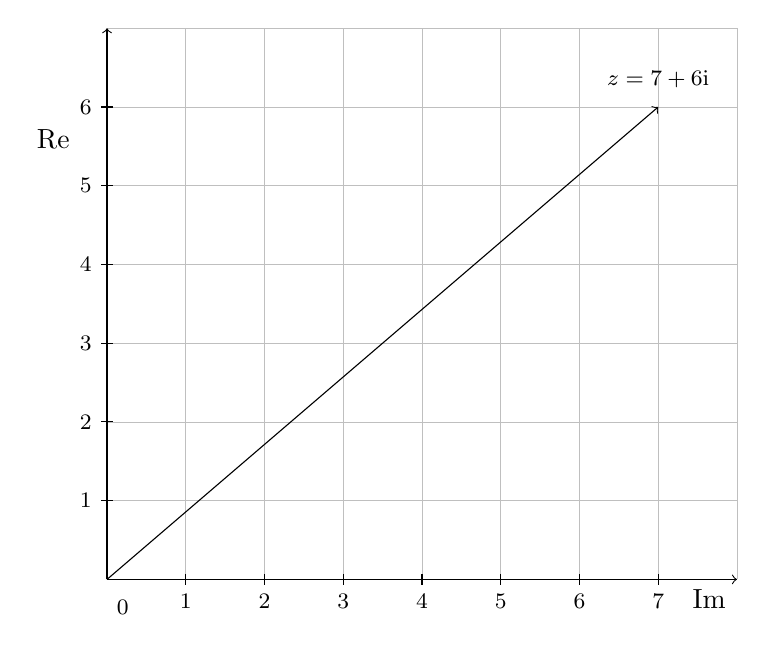
\begin{tikzpicture}

% Gitternetzlinien
\draw[xstep=1cm, ystep=1cm, very thin, color=lightgray] (0,7) grid (8,0);
% x-Achse
\draw[->] (0,0) -- (8,0) node[below,xshift=-1em] {$\mathrm{Im}$}; 
%Zahlen auf x-Achse
\foreach \x in {1,...,7}
\draw[shift={(\x,0)},color=black] (0pt,2pt) -- (0pt,-2pt) node[below] {\footnotesize $\x$};
%\foreach \x in {1,...,3}
%\draw[shift={(\x,0)},color=black] (0pt,2pt) -- (0pt,-2pt) node[below] {\footnotesize $\x$};
% y-Achse 
\draw[->] (0,0) -- (0,7) node[left,yshift=-4em,xshift=-1em] {$\mathrm{Re}$};%node[above left]
%Zahlen auf y-Achse
%\foreach \y in {-1,...,-1}
%\draw[shift={(0,\y)},color=black] (2pt,0pt) -- (-2pt,0pt) node[left] {\footnotesize $\y$};
\foreach \y in {1,...,6}
\draw[shift={(0,\y)},color=black] (2pt,0pt) -- (-2pt,0pt) node[left] {\footnotesize $\y$};
%Ursprung
\draw[color=black] (0pt,-10pt) node[right] {\footnotesize $0$};
\draw[->] (0,0) -- (7,6) node[yshift=1em]{\footnotesize $z=7+6\mathrm{i}$};


%\draw[thick,color=black] plot[samples=200, domain=2:7] 
%(\x,{\x-1}) node[below, xshift=1em]{$g(x)$};



\end{tikzpicture}\\
\end{center}
Interpretation: Darstellung als Punkt $ (7,6) $ oder als Vektor $ \binom{7}{6} $\vspace*{4mm}\\
Addition von komplexen Zahlen ist gleich der Addition der Vektoren $ \binom{5}{2}+\binom{2}{4} $.\\
$ (5+2\mathrm{i})+(2+4\mathrm{i})=(7+6\mathrm{i}) $\\
\begin{center}
	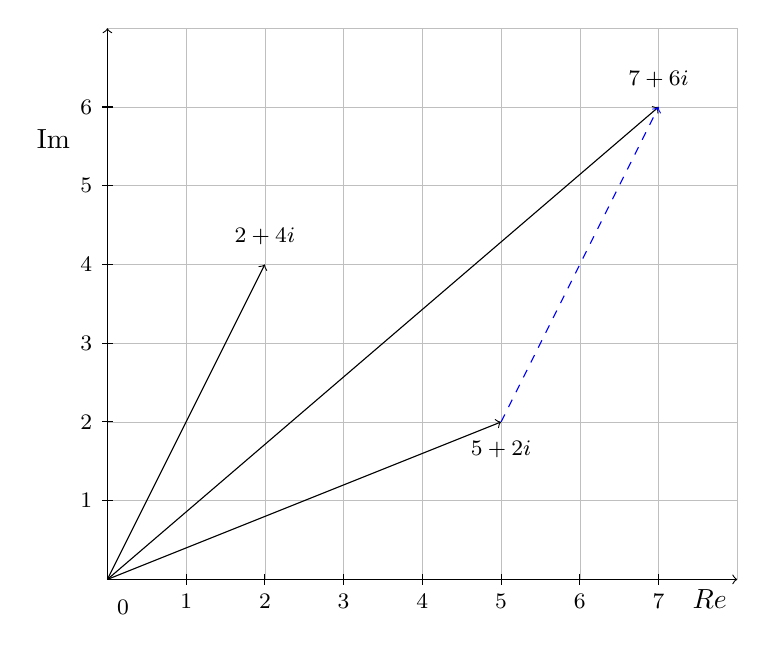
\begin{tikzpicture}
	
	% Gitternetzlinien
	\draw[xstep=1cm, ystep=1cm, very thin, color=lightgray] (0,7) grid (8,0);
	% x-Achse
	\draw[->] (0,0) -- (8,0) node[below,xshift=-1em] {$Re$}; 
	%Zahlen auf x-Achse
	\foreach \x in {1,...,7}
	\draw[shift={(\x,0)},color=black] (0pt,2pt) -- (0pt,-2pt) node[below] {\footnotesize $\x$};
	%\foreach \x in {1,...,3}
	%\draw[shift={(\x,0)},color=black] (0pt,2pt) -- (0pt,-2pt) node[below] {\footnotesize $\x$};
	% y-Achse 
	\draw[->] (0,0) -- (0,7) node[left,yshift=-4em,xshift=-1em] {$\mathrm{Im}$};%node[above left]
	%Zahlen auf y-Achse
	%\foreach \y in {-1,...,-1}
	%\draw[shift={(0,\y)},color=black] (2pt,0pt) -- (-2pt,0pt) node[left] {\footnotesize $\y$};
	\foreach \y in {1,...,6}
	\draw[shift={(0,\y)},color=black] (2pt,0pt) -- (-2pt,0pt) node[left] {\footnotesize $\y$};
	%Ursprung
	\draw[color=black] (0pt,-10pt) node[right] {\footnotesize $0$};
	\draw[->] (0,0) -- (7,6) node[yshift=1em]{\footnotesize $7+6i$};
	\draw[->] (0,0) -- (5,2) node[yshift=-1em]{\footnotesize $5+2i$};
	\draw[->] (0,0) -- (2,4) node[yshift=1em]{\footnotesize $2+4i$};
	\draw[->,color=blue,dashed] (5,2) -- (7,6) ;
	%\draw[thick,color=black] plot[samples=200, domain=2:7] 
	%(\x,{\x-1}) node[below, xshift=1em]{$g(x)$};
	
	
	
	\end{tikzpicture}\\
\end{center}
\begin{center}
	\fbox{\parbox  {80mm} {
	\begin{center}
		Betrag einer komplexen Zahl\vspace*{2mm}\\
		$  \mathbb{C}\longmapsto [0,\infty[ \subset \mathbb{R} \text{ mit } |x+\mathrm{i}y|=\sqrt{x^2+y^2} $
	\end{center}
}}
\end{center}
Beispiel:\\
$ |7+6\mathrm{i}|=\sqrt{7^2+6^2}=\sqrt{85} $\\
\begin{center}
	\fbox{\parbox  {80mm} {
	\begin{center}
		Kunjugation einer komplexen Zahl \vspace*{2mm}\\
		$  \mathbb{C}\longmapsto  \mathbb{C}\text{ mit }\overline{(x+\mathrm{i}y)}=(x-\mathrm{i}y) $
	\end{center}
}}
\end{center}
Beispiel:\vspace*{2mm}\\
$\overline{(3+3\mathrm{i})}=(3-3\mathrm{i})$\\
\begin{center}
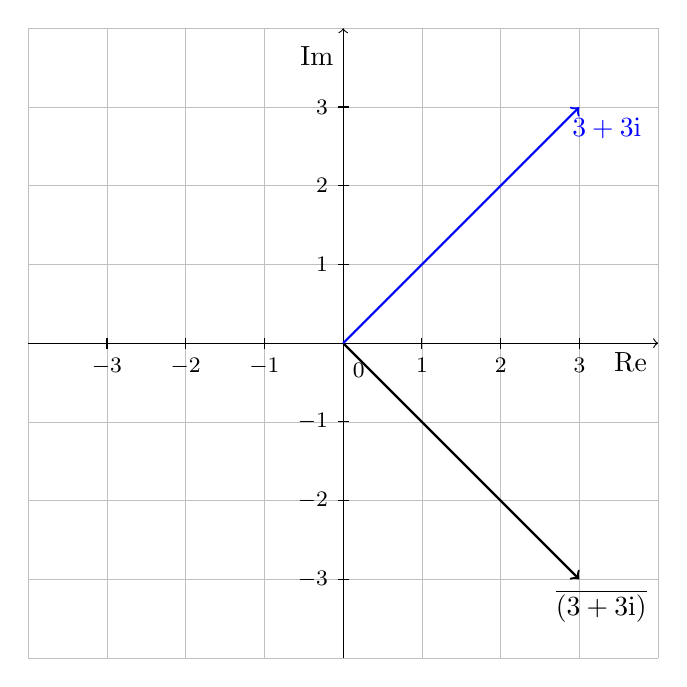
\begin{tikzpicture}

% Gitternetzlinien
\draw[xstep=1cm, ystep=1cm, very thin, color=lightgray] (-4,4) grid (4,-4);
% x-Achse
\draw[->] (-4,0) -- (4,0) node[below,xshift=-1em] {$\mathrm{Re}$}; 
%Zahlen auf x-Achse
\foreach \x in {-3,...,-1}
\draw[shift={(\x,0)},color=black] (0pt,2pt) -- (0pt,-2pt) node[below] {\footnotesize $\x$};
\foreach \x in {1,...,3}
\draw[shift={(\x,0)},color=black] (0pt,2pt) -- (0pt,-2pt) node[below] {\footnotesize $\x$};
% y-Achse 
\draw[->] (0,-4) -- (0,4) node[left,yshift=-1em] {$\mathrm{Im}$};%node[above left]
%Zahlen auf y-Achse
\foreach \y in {-3,...,-1}
\draw[shift={(0,\y)},color=black] (2pt,0pt) -- (-2pt,0pt) node[left] {\footnotesize $\y$};
\foreach \y in {1,...,3}
\draw[shift={(0,\y)},color=black] (2pt,0pt) -- (-2pt,0pt) node[left] {\footnotesize $\y$};
%Ursprung
\draw[color=black] (0pt,-10pt) node[right] {\footnotesize $0$};

\draw[thick,color=black,->] plot[samples=200, domain=0:3] 
(\x,{-1*\x}) node[below, xshift=0.8em] {$\overline{(3+3\mathrm{i})}$};

\draw[thick,color=blue,->] plot[samples=200, domain=0:3] 
(\x,{\x}) node[below, xshift=1em]{$3+3\mathrm{i}$};



\end{tikzpicture}\\
\end{center}
Die Kunjugation einer komplexen Zahl entspricht der Spiegelung des Vektors  an der Re-Achse.\\
\subsubsection{Aufgabe 1 zu Grundlagen der komplexen Zahlen }
\href{https://youtu.be/xC24jiGbXjo}{Video 05}\\
Skiziere die folgende Menge in die Gaußschene Zahlenebene:\\
\begin{align*}
\mathbb{A}= \{z \in  \mathbb{C}\;|\; 1\leq|z| \leq 4\}\cap\{z\in  \mathbb{C}\;|\; \mathrm{Re}_{(z)}\geq 1\}
\end{align*}
Zuerst für $ z=x+\mathrm{i}y $, $ |z|=\sqrt{x^2+y^2} $ und für $ \mathrm{Re}_{z}=x$ einsetzen.\\
\begin{align*}
\Leftrightarrow\mathbb{A}= \{x+\mathrm{i}y \in  \mathbb{C}\;|\; 1\leq \sqrt{x^2+y^2} \leq 4\}\cap\{x+\mathrm{i}y\in  \mathbb{C}\;|\; x\geq 1\}
\end{align*}
Zur Darstellung in die Zahlenebene benötigt man die Kreisgleichung.\\
\begin{center}
\fbox{\parbox  {60mm} {
		\begin{center}
				Kreisgleichung
		\end{center}
		\begin{align*}
		(x-x_0)^2+(y-y_0)^2=r^2\\
		\scriptscriptstyle \text{Radius }=r \text{ Mittelpunkt= }\scriptscriptstyle (x_0,y_0)
		\end{align*}
	%	$\scriptscriptstyle r \overset{\wedge}{=} \text{Radius } \text{ Mittelpunkt= }\scriptscriptstyle (x_0,y_0)  $
}}
\end{center}
Dann gilt:\\
\begin{align*}
\sqrt{(x-0)^2+(y-0)^2}=4\Leftrightarrow (x-0)^2+(y-0)^2=4^2\Rightarrow \text{ Kreis mit } r=4 \text{ vom Mittelpunkt } (0,0)\\
\end{align*}
\begin{center}
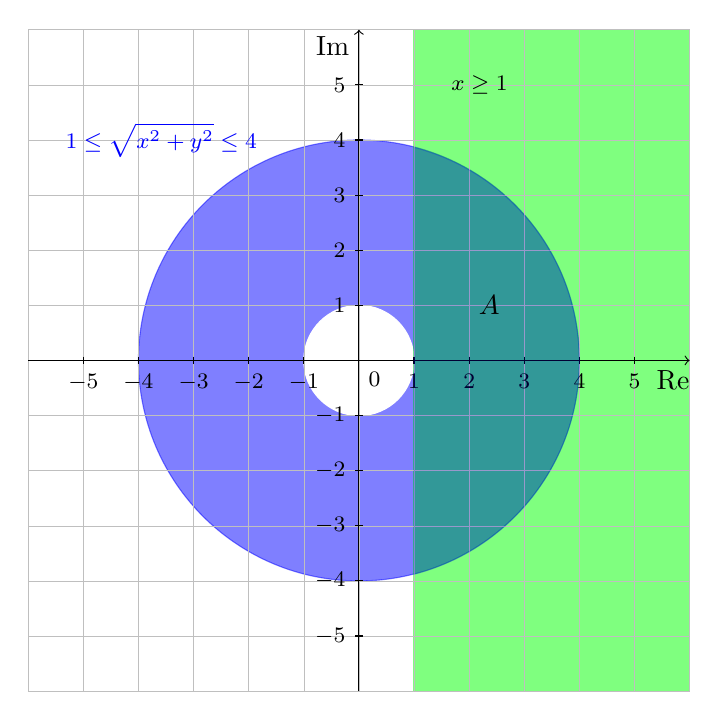
\begin{tikzpicture}[scale=.7]
\filldraw [blue,opacity=0.5] (0,0) circle (4);
\filldraw [white] (0,0) circle (1);
\filldraw [green,opacity=0.5] (1,-6) rectangle (6,6);
% Gitternetzlinien
\draw[xstep=1cm, ystep=1cm, very thin, color=lightgray] (-6,6) grid (6,-6);
% x-Achse
\draw[->] (-6,0) -- (6,0) node[below,xshift=-0.6em] {$\mathrm{Re}$}; 
%Zahlen auf x-Achse
\foreach \x in {-5,...,-1}
\draw[shift={(\x,0)},color=black] (0pt,2pt) -- (0pt,-2pt) node[below] {\footnotesize $\x$};
\foreach \x in {1,...,5}
\draw[shift={(\x,0)},color=black] (0pt,2pt) -- (0pt,-2pt) node[below] {\footnotesize $\x$};
% y-Achse 
\draw[->] (0,-6) -- (0,6) node[left,yshift=-0.6em] {$\mathrm{Im}$};%node[above left]
%Zahlen auf y-Achse
\foreach \y in {-5,...,-1}
\draw[shift={(0,\y)},color=black] (2pt,0pt) -- (-2pt,0pt) node[left] {\footnotesize $\y$};
\foreach \y in {1,...,5}
\draw[shift={(0,\y)},color=black] (2pt,0pt) -- (-2pt,0pt) node[left] {\footnotesize $\y$};
%Ursprung
\draw[color=black] (0pt,-10pt) node[right] {\footnotesize $0$};

%\draw[thick,color=black] plot[samples=200, domain=2:4] 
%(\x,{2}) node[below, xshift=-5em] {$h(x)$};

%\draw[thick,color=black] plot[samples=200, domain=-1:2] 
%(\x,{\x-1}) node[below, xshift=1em]{$g(x)$};

%\filldraw [blue,opacity=0.5] (0,0) circle (4);
%\filldraw [white,opacity=0.9] (0,0) circle (1);
%\filldraw [fill=green,draw=blue] (2,-2) rectangle (4,4);
%\filldraw[fill=cyan, draw=blue] (0,0) -- (0,0) arc (90:-90:10mm) -- (0,0);
%\filldraw[fill=cyan,draw=blue ](-1,1) -- (0,1)  arc[radius = 10mm, start angle= 0, end angle= 180];
%\draw[rotate=270,color=blue] (1,1)  arc[radius = 10mm, start angle= 0, end angle= 180];

\filldraw[blue,opacity=0.2] (1,3.88)--(1,-3.88)  arc[radius = 40mm, start angle= -75.5, end angle= 75.5];
\draw[color=black] (2,1) node[right] {$\mathbb{A}$};
\draw[color=blue] (-5.5,4) node[right] {\footnotesize $1\leq\sqrt{x^2+y^2}\leq4$};
\draw[color=black] (1.5,5) node[right] {\footnotesize $x\geq1$};
\end{tikzpicture}\\
\end{center}
\subsubsection{Aufgabe 2 zu Grundlagen der komplexen Zahlen}
\href{https://youtu.be/0TRhS_AU7g0}{Video 06}\\
Skiziere die folgende Menge in die Gaußschene Zahlenebene:\\
\begin{align*}
\mathbb{A}=\{z \in \mathbb{Z}\;|\;|\mathrm{Im}(z)|\leq 2\cdot|\mathrm{Re}(z)|\}\cap\{z\in \mathbb{C}\;|\;|z|\leq 1 \}
\end{align*}
Zuerst für $ z=x+\mathrm{i}y $, $ \mathrm{Im}(z)=y $ und $ \mathrm{Re}(z)=x$ und $ |z|=\sqrt{x^2+y^2} $ ersetzen.\\
\begin{align*}
\mathbb{A}=\{x+\mathrm{i}y \in \mathbb{Z}\;|\;|y|\leq 2\cdot|x|\}\cap\{x+\mathrm{i}y\in \mathbb{C}\;|\;\sqrt{x^2+y^2}\leq 1 \}
\end{align*}
Vorgehensweise:\\
\textbullet \;\;Zeichne die Menge $|y|\leq 2\cdot|x| $im I.Quatranten:\\
\begin{quote}
Es gilt: $ y\leq2x  $\\	
Zeichne zuerst die Menge: $ y=2x $ \\
Wähle einen Punkt für die, die Gleichung $ y\leq2x $ gilt:\\Für den  Punkt$P=(1,1)  $ erhält man $1\leq2\cdot1  $, deshalb ist die Menge unterhalb der Geraden.\\

\begin{center}
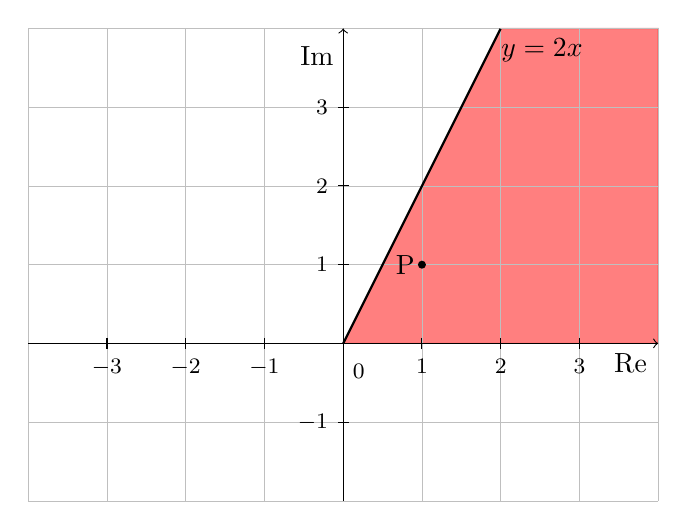
\begin{tikzpicture}
\filldraw [red,opacity=0.5] (0,0)--(1,2)--(2,4)--(4,4)--(4,0)--(0,0);
% Gitternetzlinien
\draw[xstep=1cm, ystep=1cm, very thin, color=lightgray] (-4,4) grid (4,-2);
% x-Achse
\draw[->] (-4,0) -- (4,0) node[below,xshift=-1em] {$\mathrm{Re}$}; 
%Zahlen auf x-Achse
\foreach \x in {-3,...,-1}
\draw[shift={(\x,0)},color=black] (0pt,2pt) -- (0pt,-2pt) node[below] {\footnotesize $\x$};
\foreach \x in {1,...,3}
\draw[shift={(\x,0)},color=black] (0pt,2pt) -- (0pt,-2pt) node[below] {\footnotesize $\x$};
% y-Achse 
\draw[->] (0,-2) -- (0,4) node[left,yshift=-1em] {$\mathrm{Im}$};%node[above left]
%Zahlen auf y-Achse
\foreach \y in {-1,...,-1}
\draw[shift={(0,\y)},color=black] (2pt,0pt) -- (-2pt,0pt) node[left] {\footnotesize $\y$};
\foreach \y in {1,...,3}
\draw[shift={(0,\y)},color=black] (2pt,0pt) -- (-2pt,0pt) node[left] {\footnotesize $\y$};
%Ursprung
\draw[color=black] (0pt,-10pt) node[right] {\footnotesize $0$};

\draw[thick,color=black] plot[samples=200, domain=0:2] 
(\x,{2*\x}) node[below, xshift=1.5em] {$y=2x$};





\fill [black] (1,1) circle (.051cm) ;
\draw (1,1) node[xshift=-0.6em]{P};





\end{tikzpicture}\\
\end{center}
\end{quote}
\textbullet \;\;Zeichne die Menge im II.Quatranten:\\

\begin{quote}
Es gilt: $ y\leq-2x  $\\	
Zeichne zuerst die Menge: $ y=-2x $ \\
Wähle einen Punkt für die, die Gleichung $ y\leq-2x $ gilt:\\Für den  Punkt $P=(-1,1)  $ erhält man $-1\leq2\cdot1  $, deshalb ist die Menge unterhalb der Geraden.\\
\begin{center}
	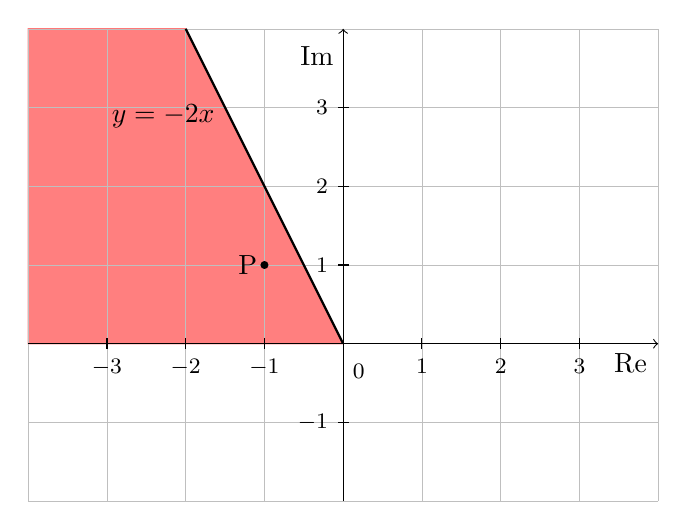
\begin{tikzpicture}
	\filldraw [red,opacity=0.5] (0,0)--(-1,2)--(-2,4)--(-4,4)--(-4,0)--(0,0);
	% Gitternetzlinien
	\draw[xstep=1cm, ystep=1cm, very thin, color=lightgray] (-4,4) grid (4,-2);
	% x-Achse
	\draw[->] (-4,0) -- (4,0) node[below,xshift=-1em] {$\mathrm{Re}$}; 
	%Zahlen auf x-Achse
	\foreach \x in {-3,...,-1}
	\draw[shift={(\x,0)},color=black] (0pt,2pt) -- (0pt,-2pt) node[below] {\footnotesize $\x$};
	\foreach \x in {1,...,3}
	\draw[shift={(\x,0)},color=black] (0pt,2pt) -- (0pt,-2pt) node[below] {\footnotesize $\x$};
	% y-Achse 
	\draw[->] (0,-2) -- (0,4) node[left,yshift=-1em] {$\mathrm{Im}$};%node[above left]
	%Zahlen auf y-Achse
	\foreach \y in {-1,...,-1}
	\draw[shift={(0,\y)},color=black] (2pt,0pt) -- (-2pt,0pt) node[left] {\footnotesize $\y$};
	\foreach \y in {1,...,3}
	\draw[shift={(0,\y)},color=black] (2pt,0pt) -- (-2pt,0pt) node[left] {\footnotesize $\y$};
	%Ursprung
	\draw[color=black] (0pt,-10pt) node[right] {\footnotesize $0$};
	
	\draw[thick,color=black] plot[samples=200, domain=-2:0] 
	(\x,{-2*\x}) node[below, xshift=-6.5em, yshift=9em] {$y=-2x$};
	
	
	
	
	
	\fill [black] (-1,1) circle (.051cm) ;
	\draw (-1,1) node[xshift=-0.6em]{P};
	
	
	
	
	
	\end{tikzpicture}\\
\end{center}
\end{quote}
\textbullet \;\;Zeichne die Menge im III.Quatranten:\\
\begin{quote}
Es gilt: $ -y\leq-2x  $\\	
Zeichne zuerst die Menge: $ -y=-2x $ \\
Wähle einen Punkt für die, die Gleichung $ -y\leq-2x $ gilt:\\Für den  Punkt $P=(-1,-1)  $ erhält man $1\leq-2\cdot-1  $, deshalb ist die Menge oberhalb der Geraden.\\
\begin{center}
	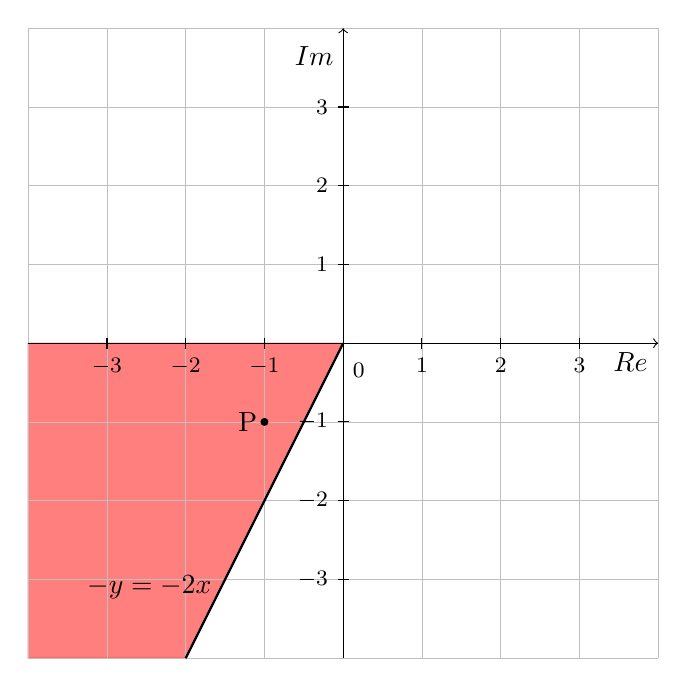
\begin{tikzpicture}
	\filldraw [red,opacity=0.5] (0,0)--(-4,0)--(-4,-4)--(-2,-4)--(0,0);
	% Gitternetzlinien
	\draw[xstep=1cm, ystep=1cm, very thin, color=lightgray] (-4,-4) grid (4,4);
	% x-Achse
	\draw[->] (-4,0) -- (4,0) node[below,xshift=-1em] {$Re$}; 
	%Zahlen auf x-Achse
	\foreach \x in {-3,...,-1}
	\draw[shift={(\x,0)},color=black] (0pt,2pt) -- (0pt,-2pt) node[below] {\footnotesize $\x$};
	\foreach \x in {1,...,3}
	\draw[shift={(\x,0)},color=black] (0pt,2pt) -- (0pt,-2pt) node[below] {\footnotesize $\x$};
	% y-Achse 
	\draw[->] (0,-4) -- (0,4) node[left,yshift=-1em] {$Im$};%node[above left]
	%Zahlen auf y-Achse
	\foreach \y in {-1,...,-3}
	\draw[shift={(0,\y)},color=black] (2pt,0pt) -- (-2pt,0pt) node[left] {\footnotesize $\y$};
	\foreach \y in {1,...,3}
	\draw[shift={(0,\y)},color=black] (2pt,0pt) -- (-2pt,0pt) node[left] {\footnotesize $\y$};
	%Ursprung
	\draw[color=black] (0pt,-10pt) node[right] {\footnotesize $0$};
	
	\draw[thick,color=black] plot[samples=200, domain=-2:0] 
	(\x,{2*\x}) node[below, xshift=-7em, yshift=-8em] {$-y=-2x$};
	
	
	
	
	
	\fill [black] (-1,-1) circle (.051cm) ;
	\draw (-1,-1) node[xshift=-0.6em]{P};
	
	
	
	
	
	\end{tikzpicture}\\
\end{center}
\end{quote}
\newpage
\textbullet \;\;Zeichne die Menge im IV.Quatranten:\\

\begin{quote}
	Es gilt: $ -y\leq 2x  $\\	
	Zeichne zuerst die Menge: $ -y= 2x $ \\
	Wähle einen Punkt für die, die Gleichung $ -y\leq 2x $ gilt:\\Für den  Punkt $P=(1,-1)  $ erhält man $1\leq2\cdot1  $, deshalb ist die Menge oberhalb der Geraden.\\
	\begin{center}
		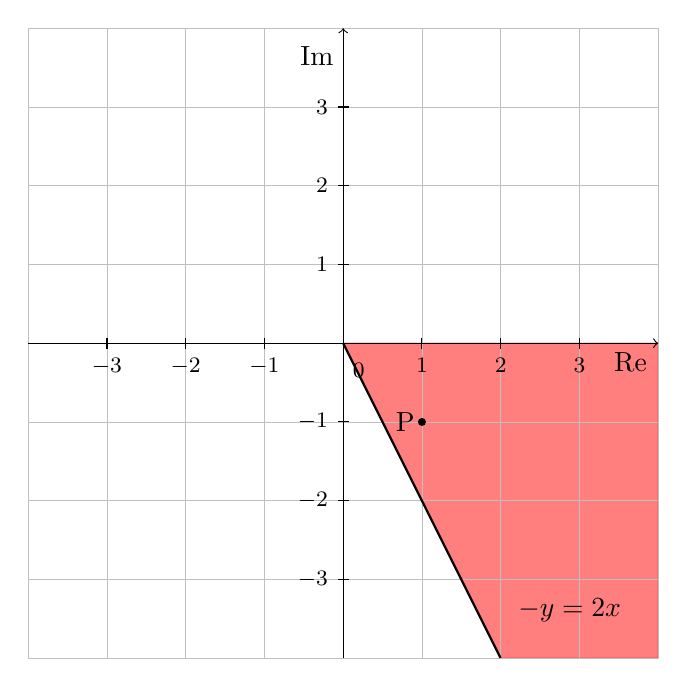
\begin{tikzpicture}
		\filldraw [red,opacity=0.5] (0,0)--(4,0)--(4,-4)--(2,-4)--(0,0);
		% Gitternetzlinien
		\draw[xstep=1cm, ystep=1cm, very thin, color=lightgray] (-4,4) grid (4,-4);
		% x-Achse
		\draw[->] (-4,0) -- (4,0) node[below,xshift=-1em] {$\mathrm{Re}$}; 
		%Zahlen auf x-Achse
		\foreach \x in {-3,...,-1}
		\draw[shift={(\x,0)},color=black] (0pt,2pt) -- (0pt,-2pt) node[below] {\footnotesize $\x$};
		\foreach \x in {1,...,3}
		\draw[shift={(\x,0)},color=black] (0pt,2pt) -- (0pt,-2pt) node[below] {\footnotesize $\x$};
		% y-Achse 
		\draw[->] (0,-4) -- (0,4) node[left,yshift=-1em] {$\mathrm{Im}$};%node[above left]
		%Zahlen auf y-Achse
		\foreach \y in {-1,...,-3}
		\draw[shift={(0,\y)},color=black] (2pt,0pt) -- (-2pt,0pt) node[left] {\footnotesize $\y$};
		\foreach \y in {1,...,3}
		\draw[shift={(0,\y)},color=black] (2pt,0pt) -- (-2pt,0pt) node[left] {\footnotesize $\y$};
		%Ursprung
		\draw[color=black] (0pt,-10pt) node[right] {\footnotesize $0$};
		
		\draw[thick,color=black] plot[samples=200, domain=0:2] 
		(\x,{-2*\x}) node[below, xshift=2.5em, yshift=2.5em] {$-y=2x$};
		
		
		
		
		
		\fill [black] (1,-1) circle (.051cm) ;
		\draw (1,-1) node[xshift=-0.6em]{P};
		
		
		
		
		
		\end{tikzpicture}\\
	\end{center}
\end{quote}
Die gesamte Menge $|y|\leq 2\cdot|x|$ ist dann:\\
\begin{center}
	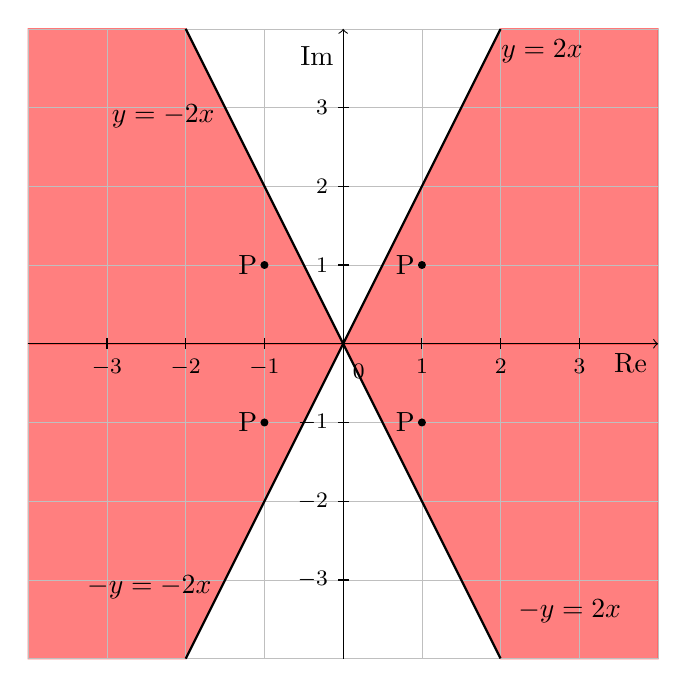
\begin{tikzpicture}
	\filldraw [red,opacity=0.5] (0,0)--(4,0)--(4,-4)--(2,-4)--(0,0);
	\filldraw [red,opacity=0.5] (0,0)--(-1,2)--(-2,4)--(-4,4)--(-4,0)--(0,0);
	\filldraw [red,opacity=0.5] (0,0)--(1,2)--(2,4)--(4,4)--(4,0)--(0,0);
	\filldraw [red,opacity=0.5] (0,0)--(-4,0)--(-4,-4)--(-2,-4)--(0,0);
	% Gitternetzlinien
	\draw[xstep=1cm, ystep=1cm, very thin, color=lightgray] (-4,-4) grid (4,4);
	% x-Achse
	\draw[->] (-4,0) -- (4,0) node[below,xshift=-1em] {$\mathrm{Re}$}; 
	%Zahlen auf x-Achse
	\foreach \x in {-3,...,-1}
	\draw[shift={(\x,0)},color=black] (0pt,2pt) -- (0pt,-2pt) node[below] {\footnotesize $\x$};
	\foreach \x in {1,...,3}
	\draw[shift={(\x,0)},color=black] (0pt,2pt) -- (0pt,-2pt) node[below] {\footnotesize $\x$};
	% y-Achse 
	\draw[->] (0,-4) -- (0,4) node[left,yshift=-1em] {$\mathrm{Im}$};%node[above left]
	%Zahlen auf y-Achse
	\foreach \y in {-1,...,-3}
	\draw[shift={(0,\y)},color=black] (2pt,0pt) -- (-2pt,0pt) node[left] {\footnotesize $\y$};
	\foreach \y in {1,...,3}
	\draw[shift={(0,\y)},color=black] (2pt,0pt) -- (-2pt,0pt) node[left] {\footnotesize $\y$};
	%Ursprung
	\draw[color=black] (0pt,-10pt) node[right] {\footnotesize $0$};
	
	\draw[thick,color=black] plot[samples=200, domain=-2:0] 
	(\x,{2*\x}) node[below, xshift=-7em, yshift=-8em] {$-y=-2x$};
	
	\draw[thick,color=black] plot[samples=200, domain=-2:0] 
	(\x,{-2*\x}) node[below, xshift=-6.5em, yshift=9em] {$y=-2x$};
	
	\draw[thick,color=black] plot[samples=200, domain=0:2] 
	(\x,{2*\x}) node[below, xshift=1.5em] {$y=2x$};
	
	\draw[thick,color=black] plot[samples=200, domain=0:2] 
	(\x,{-2*\x}) node[below, xshift=2.5em, yshift=2.5em] {$-y=2x$};
	\fill [black] (-1,-1) circle (.051cm) ;
	\draw (-1,-1) node[xshift=-0.6em]{P};
	
	\fill [black] (-1,1) circle (.051cm) ;
	\draw (-1,1) node[xshift=-0.6em]{P};
	
	\fill [black] (1,1) circle (.051cm) ;
	\draw (1,1) node[xshift=-0.6em]{P};
		\fill [black] (1,-1) circle (.051cm) ;
	\draw (1,-1) node[xshift=-0.6em]{P};
	\end{tikzpicture}\\
\end{center}
\textbullet\;\;Zeichne die Menge $ \sqrt{x^2+y^2}\leq 1 $\\
\begin{quote}
	\begin{align*}
	\sqrt{x^2+y^2}\leq1\Leftrightarrow \sqrt{(x-x_0)^2+(y-y_0)^2}\leq 1\Leftrightarrow (x-x_0)^2+(y-y_0)^2=1^1
	\end{align*}
\end{quote}
Zeichne nun $ (x-x_0)^2+(y-y_0)^2=1 $ , die gesamte Menge ist dann von $ r=1 $ bis $ r=0 $.\\


\begin{center}
	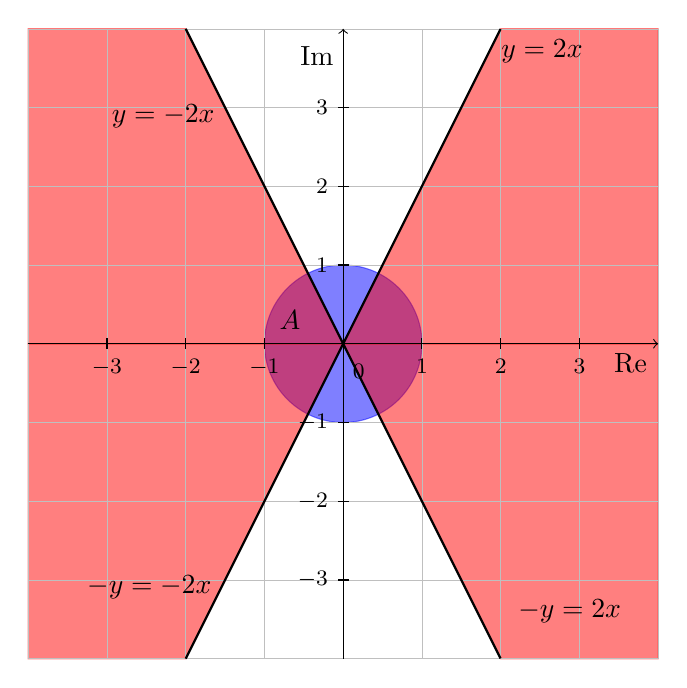
\begin{tikzpicture}
	\filldraw [blue,opacity=0.5] (0,0) circle (1);
	\filldraw [red,opacity=0.5] (0,0)--(4,0)--(4,-4)--(2,-4)--(0,0);
	\filldraw [red,opacity=0.5] (0,0)--(-1,2)--(-2,4)--(-4,4)--(-4,0)--(0,0);
	\filldraw [red,opacity=0.5] (0,0)--(1,2)--(2,4)--(4,4)--(4,0)--(0,0);
	\filldraw [red,opacity=0.5] (0,0)--(-4,0)--(-4,-4)--(-2,-4)--(0,0);
	% Gitternetzlinien
	\draw[xstep=1cm, ystep=1cm, very thin, color=lightgray] (-4,-4) grid (4,4);
	% x-Achse
	\draw[->] (-4,0) -- (4,0) node[below,xshift=-1em] {$\mathrm{Re}$}; 
	%Zahlen auf x-Achse
	\foreach \x in {-3,...,-1}
	\draw[shift={(\x,0)},color=black] (0pt,2pt) -- (0pt,-2pt) node[below] {\footnotesize $\x$};
	\foreach \x in {1,...,3}
	\draw[shift={(\x,0)},color=black] (0pt,2pt) -- (0pt,-2pt) node[below] {\footnotesize $\x$};
	% y-Achse 
	\draw[->] (0,-4) -- (0,4) node[left,yshift=-1em] {$\mathrm{Im}$};%node[above left]
	%Zahlen auf y-Achse
	\foreach \y in {-1,...,-3}
	\draw[shift={(0,\y)},color=black] (2pt,0pt) -- (-2pt,0pt) node[left] {\footnotesize $\y$};
	\foreach \y in {1,...,3}
	\draw[shift={(0,\y)},color=black] (2pt,0pt) -- (-2pt,0pt) node[left] {\footnotesize $\y$};
	%Ursprung
	\draw[color=black] (0pt,-10pt) node[right] {\footnotesize $0$};
	
	\draw[thick,color=black] plot[samples=200, domain=-2:0] 
	(\x,{2*\x}) node[below, xshift=-7em, yshift=-8em] {$-y=-2x$};
	
	\draw[thick,color=black] plot[samples=200, domain=-2:0] 
	(\x,{-2*\x}) node[below, xshift=-6.5em, yshift=9em] {$y=-2x$};
	
	\draw[thick,color=black] plot[samples=200, domain=0:2] 
	(\x,{2*\x}) node[below, xshift=1.5em] {$y=2x$};
	
	\draw[thick,color=black] plot[samples=200, domain=0:2] 
	(\x,{-2*\x}) node[below, xshift=2.5em, yshift=2.5em] {$-y=2x$};
	
	
	
	
	
	
	\draw (-0.5,0.3) node[xshift=-0.5em]{$\mathbb{A}$};
	\end{tikzpicture}\\
\end{center}
\subsubsection{Aufgabe 1 zur Darstellung komplexer Zahlen in kartesischen Koordinaten}
\href{https://youtu.be/FL3zN9eSh_c}{Video 07}\\
Stelle folgende komplexe Zahl in der Form $ x+\mathrm{i}y\; |\; x,y \in \mathbb{R}$ dar:\\
\begin{align*}
\frac{8-\mathrm{i}}{5-1}
\end{align*}
Durch Erweiterung mit $ (5+1) $ und Ausnützung der 3. binomischen Formel erhält man:\\
\begin{align*}
\frac{8-\mathrm{i}}{5-\mathrm{i}}=\frac{(8-\mathrm{i})(5+\mathrm{i})}{(5-\mathrm{i})(5+\mathrm{i})}=\frac{40+8\mathrm{i}-5\mathrm{i}-\mathrm{i}^2}{5^2-\mathrm{i}^2}=\frac{40+3\mathrm{i}-(-1)}{25-(-1)}=\frac{41+3\mathrm{i}}{26}=\frac{41}{26}+\mathrm{i}\frac{3}{26} \text{ mit }x \in \mathbb{R}
\end{align*}
\subsubsection{Aufgabe 2 zur Darstellung komplexer Zahlen in kartesischen Koordinaten}
\href{https://youtu.be/fm9W_BQeuOA}{Video 08}\\
Stelle folgende komplexe Zahl in der Form $ x+\mathrm{i}y $ mit $ x,y \in \mathbb{R} $ dar.\\
\begin{align*}
\sum\limits_{n=1}^{493836} \mathrm{i}^n\;\; \;\; n\in\mathbb{N}
\end{align*}
Für die Summe gilt doch:
\begin{align*}
\sum\limits_{n=1}^{493836} \mathrm{i}^n= \mathrm{i}^1+\mathrm{i}^2+\mathrm{i}^3\ldots 493836\\
\end{align*}
\newpage
\noindent
Es gilt:\\
\begin{align*}
&\mathrm{i}^1=\mathrm{i}\\
&\mathrm{i}^2=-\mathrm{i}\\
&\mathrm{i}^4=\mathrm{i}^2\cdot \mathrm{i}^2=(-1)(-1)=1\\
&\sum\limits_{n=1}^{493836} \mathrm{i}^n= \mathrm{i}^1+\mathrm{i}^2+\mathrm{i}^3+\mathrm{i}^4+\underbrace {\mathrm{i}^5}_{=\mathrm{i}^4\cdot \mathrm{i}^1=\mathrm{i}^1}+\underbrace {\mathrm{i}^6}_{=\mathrm{i}^4\cdot \mathrm{i}^2=\mathrm{i}^2}+\underbrace {\mathrm{i}^7}_{=\mathrm{i}^4+\mathrm{i}^3=\mathrm{i}^3}+\underbrace {\mathrm{i}^8}_{\mathrm{i}^4\cdot \mathrm{i}^4=1=\mathrm{i}^4}+\underbrace {\mathrm{i}^9}_{=\mathrm{i}^4\cdot \mathrm{i}^4\cdot \mathrm{i}=\mathrm{i}^1}\ldots\\
\end{align*}
Die ersten Summen 1-4 sind also gleich mit den Summen 5-8 und den Summen 9-12 usw..\\
Es gilt dann:\\
\begin{align*}
& \sum\limits_{n=1}^{493836} \mathrm{i}^n=\sum\limits_{n=1}^{\frac{493836}{4}}(\mathrm{i}+\mathrm{i}^2+\mathrm{i}^3+\mathrm{i}^4)\\
&\hspace{1.4cm}=\frac{493836}{4}(\mathrm{i}+\mathrm{i}^2+\mathrm{i}^3+\mathrm{i}^4)=\frac{493836}{4}(\mathrm{i}+(-1)+(-1\cdot \mathrm{i})+1)=\frac{493836}{4}\cdot 0\\
&\hspace{1.4cm}=0+0\mathrm{i}\\
\end{align*}
\subsection{Polarkoordinaten komplexer Zahlen}
\subsubsection{Polarkoordinaten komplexer Zahlen - Herleitung}
\href{https://youtu.be/8uVqLVXBXL4}{Video 09}\\
Für $ z=x+\mathrm{i}y $ und $ |z|=1 $ gilt:\\
\begin{align*}
&z=\cos(\alpha)+i\cdot \sin(\alpha) \text{ für }|z|=1\\
\end{align*}
\begin{center}

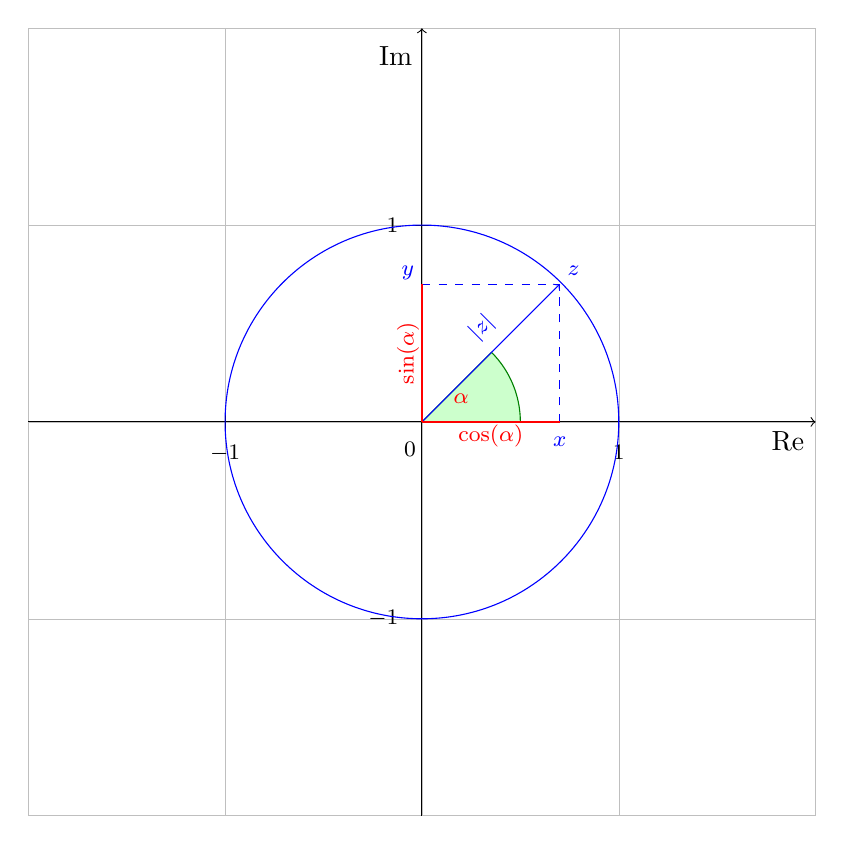
\begin{tikzpicture}[scale=2.5]

% Gitternetzlinien
\draw[xstep=1cm, ystep=1cm, very thin, color=lightgray] (-2,-2) grid (2,2);
% x-Achse
\draw[->] (-2,0) -- (2,0) node[below,xshift=-1em] {$\mathrm{Re}$}; 
%Zahlen auf x-Achse
\foreach \x in {-1,...,-1}
\draw[shift={(\x,0)},color=black] (0pt,2pt) -- (0pt,-2pt) node[below] {\footnotesize $\x$};
\foreach \x in {1,...,1}
\draw[shift={(\x,0)},color=black] (0pt,2pt) -- (0pt,-2pt) node[below] {\footnotesize $\x$};
% y-Achse 
\draw[->] (0,-2) -- (0,2) node[left,yshift=-1em] {$\mathrm{Im}$};%node[above left]
%Zahlen auf y-Achse
\foreach \y in {-1,...,-1}
\draw[shift={(0,\y)},color=black] (2pt,0pt) -- (-2pt,0pt) node[left] {\footnotesize $\y$};
\foreach \y in {1,...,1}
\draw[shift={(0,\y)},color=black] (2pt,0pt) -- (-2pt,0pt) node[left] {\footnotesize $\y$};
%Ursprung
%\draw[color=black] (0pt,-10pt) node[right] {\footnotesize $0$};
	\draw[color=black] (-4pt,-4pt) node[right] {\footnotesize $0$};
%\draw[thick,color=black] plot[samples=200, domain=2:4] 
%(\x,{2}) node[below, xshift=-5em] {$h(x)$};

%\draw[thick,color=black] plot[samples=200, domain=-1:2] 
%(\x,{\x-1}) node[below, xshift=1em]{$g(x)$};

\draw [blue] (0,0) circle (1);
\filldraw[fill=green!20,draw=green!50!black] (0,0) -- (5mm,0mm) arc (0:45:5mm) -- cycle; 
\draw [blue,->] (0,0)-.(0.7,0.7)node[below,xshift= 0.5em,yshift=1em] {\footnotesize $z$};
\draw [blue,dashed] (0,.7)-.(0.7,0.7);
\draw [blue,dashed] (0.7,0)-.(0.7,0.7);
\draw [blue] (0.7,0) node[below,xshift= 0em,yshift=-0.2em] {\footnotesize $x$};
\draw [blue] (0.3,0.3) node[below,xshift= -0.5em,yshift=1.8em,rotate=45] {\footnotesize $|z|$};
\draw [blue] (0,0.7) node[below,xshift=- 0.51em,yshift=1em] {\footnotesize $y$};


\draw [red,thick] (0,0)-.(0.7,0) node[midway,xshift= 0em,yshift=-0.5em] {\footnotesize $\cos(\alpha)$};
\draw [red,thick] (0,0)-.(0,0.7) node[midway,xshift= -0.50em,yshift=-0em,rotate=90] {\footnotesize $\sin(\alpha)$};
\draw [red] (0.2,0.2) node[xshift= 0em,yshift=-0.6em,rotate=0] {\footnotesize $\alpha$};
\end{tikzpicture}\\
\end{center}
\newpage
\noindent
Für $ z \in \mathbb{C} $ beliebig gilt:\\
\begin{align*}
z=x+\mathrm{i}y&=|z|\cos(\alpha)+|z|\;i\;\sin(\alpha)\\
&=|z|(\cos(\alpha)+\mathrm{i} \; \sin(\alpha))
\end{align*}
\begin{center}

\fbox{\parbox  {70mm} {
		\begin{align*}
		z=|z|(\cos(\alpha)+\mathrm{i}\; \sin(\alpha))
		\text{  für } \alpha \in [0,2\pi[
		\end{align*}
}}
\end{center}
\begin{center}

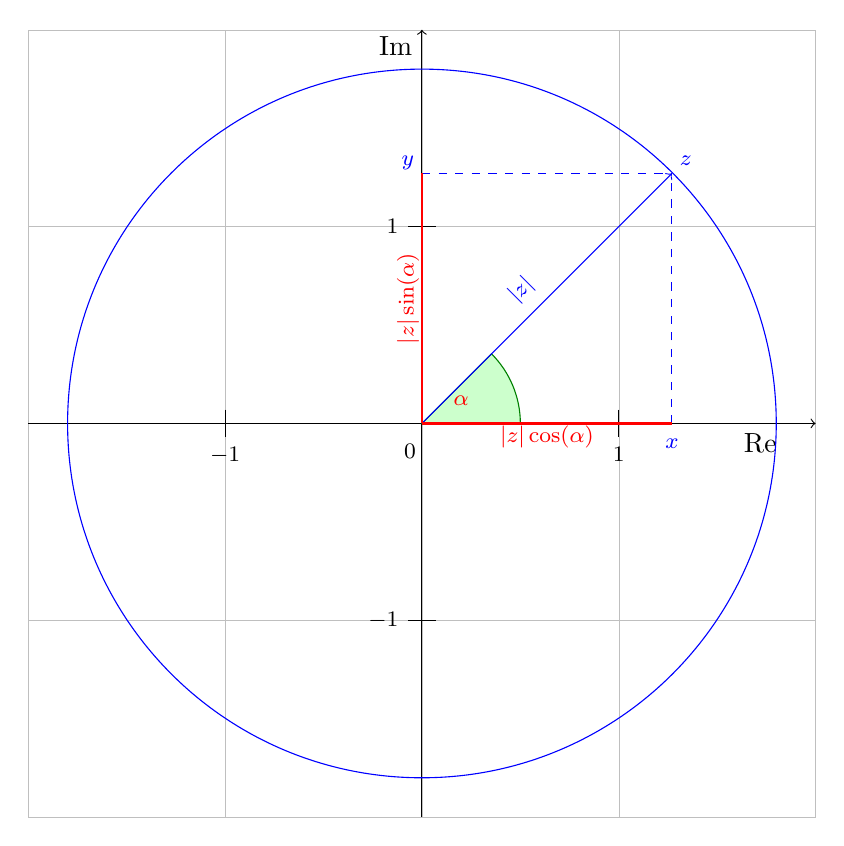
\begin{tikzpicture}[scale=2.5]

% Gitternetzlinien
\draw[xstep=1cm, ystep=1cm, very thin, color=lightgray] (-2,-2) grid (2,2);
% x-Achse
\draw[->] (-2,0) -- (2,0) node[below,xshift=-2em] {$\mathrm{Re}$}; 
%Zahlen auf x-Achse
\foreach \x in {-1,...,-1}
\draw[shift={(\x,0)},color=black] (0pt,2pt) -- (0pt,-2pt) node[below] {\footnotesize $\x$};
\foreach \x in {1,...,1}
\draw[shift={(\x,0)},color=black] (0pt,2pt) -- (0pt,-2pt) node[below] {\footnotesize $\x$};
% y-Achse 
\draw[->] (0,-2) -- (0,2) node[left,yshift=-0.6em] {$\mathrm{Im}$};%node[above left]
%Zahlen auf y-Achse
\foreach \y in {-1,...,-1}
\draw[shift={(0,\y)},color=black] (2pt,0pt) -- (-2pt,0pt) node[left] {\footnotesize $\y$};
\foreach \y in {1,...,1}
\draw[shift={(0,\y)},color=black] (2pt,0pt) -- (-2pt,0pt) node[left] {\footnotesize $\y$};
%Ursprung
%\draw[color=black] (0pt,-10pt) node[right] {\footnotesize $0$};
	\draw[color=black] (-4pt,-4pt) node[right] {\footnotesize $0$};
%\draw[thick,color=black] plot[samples=200, domain=2:4] 
%(\x,{2}) node[below, xshift=-5em] {$h(x)$};

%\draw[thick,color=black] plot[samples=200, domain=-1:2] 
%(\x,{\x-1}) node[below, xshift=1em]{$g(x)$};

\draw [blue] (0,0) circle (1.8);
\filldraw[fill=green!20,draw=green!50!black] (0,0) -- (5mm,0mm) arc (0:45:5mm) -- cycle; 
\draw [blue,->] (0,0)-.(1.27,1.27)node[below,xshift= 0.5em,yshift=1em] {\footnotesize $z$};
\draw [blue,dashed] (0,1.27)-.(1.27,1.27);
\draw [blue,dashed] (1.27,0)-.(1.27,1.27);
\draw [blue] (1.27,0) node[below,xshift= 0em,yshift=-0.2em] {\footnotesize $x$};
\draw [blue] (0.5,0.5) node[below,xshift= -0.5em,yshift=1.8em,rotate=45] {\footnotesize $|z|$};
\draw [blue] (0,1.27) node[below,xshift=- 0.51em,yshift=1em] {\footnotesize $y$};


\draw [red,thick] (0,0)-.(1.27,0) node[midway,xshift= 0em,yshift=-0.5em] {\footnotesize $|z|\cos(\alpha)$};
\draw [red,thick] (0,0)-.(0,1.27) node[midway,xshift= -0.50em,yshift=0em,rotate=90] {\footnotesize $|z|\sin(\alpha)$};
\draw [red] (0.2,0.2) node[xshift= 0em,yshift=-0.6em,rotate=0] {\footnotesize $\alpha$};
\end{tikzpicture}\\
\end{center}
Beispiel:\\
\textbullet \;\;$ z_1=1=1+0\mathrm{i}=|1|(1+0\mathrm{i}) =1(\cos(0) +\mathrm{i}\;\sin(0))$\\
\textbullet \;\;$ z_2=\mathrm{i}=0+1\mathrm{i}\;=|1|(0+1\;\mathrm{i})=1(\cos(\frac{\pi}{2})+\mathrm{i}\;\sin(\frac{\pi}{2})) $\\
\textbullet \;\;$ z_3=1,5+1,6\;\mathrm{i}=|\sqrt{1,5^2+1,6^2}|(\underbrace {\scriptstyle\frac{1,5}{2,19}}_{=\cos(\alpha)}+\mathrm{i}\underbrace {\scriptscriptstyle\frac{1,6}{2,19}}_{=\sin(\alpha)})=2,19(\cos(0,684)+\mathrm{i}\;\sin(0,730))$\\
\begin{center}
	
	\begin{tikzpicture}[scale=2.5]
	
	% Gitternetzlinien
	\draw[xstep=1cm, ystep=1cm, very thin, color=lightgray] (-2,-2) grid (2,2);
	% x-Achse
	\draw[->] (-2,0) -- (2,0) node[below,xshift=-1em] {$\mathrm{Re}$}; 
	%Zahlen auf x-Achse
	\foreach \x in {-1,...,-1}
	\draw[shift={(\x,0)},color=black] (0pt,2pt) -- (0pt,-2pt) node[below] {\footnotesize $\x$};
	\foreach \x in {1,...,1}
	\draw[shift={(\x,0)},color=black] (0pt,2pt) -- (0pt,-2pt) node[below] {\footnotesize $\x$};
	% y-Achse 
	\draw[->] (0,-2) -- (0,2) node[left,yshift=-1em] {$\mathrm{Im}$};%node[above left]
	%Zahlen auf y-Achse
	\foreach \y in {-1,...,-1}
	\draw[shift={(0,\y)},color=black] (2pt,0pt) -- (-2pt,0pt) node[left] {\footnotesize $\y$};
	\foreach \y in {1,...,1}
	\draw[shift={(0,\y)},color=black] (2pt,0pt) -- (-2pt,0pt) node[left] {\footnotesize $\y$};
	%Ursprung
	%\draw[color=black] (0pt,-10pt) node[right] {\footnotesize $0$};
		\draw[color=black] (-4pt,-4pt) node[right] {\footnotesize $0$};
	%\draw[thick,color=black] plot[samples=200, domain=2:4] 
	%(\x,{2}) node[below, xshift=-5em] {$h(x)$};
	
	%\draw[thick,color=black] plot[samples=200, domain=-1:2] 
	%(\x,{\x-1}) node[below, xshift=1em]{$g(x)$};
	
	
	\draw [green,->,thick] (0,0)-.(0,1)node[below,xshift= 0.5em,yshift=1em] {\footnotesize $z_2$};
	\draw [blue,->,thick] (0,0)-.(1,0)node[below,xshift= 0.5em,yshift=1em] {\footnotesize $z_1$};
	
	\draw [red,->,thick] (0,0)-.(1.5,1.6)node[below,xshift= 0.5em,yshift=1em] {\footnotesize $z_3$};
	\draw [red,dashed] (1.5,0)- -(1.5,1.6);
	\draw [red,dashed] (0,1.6)- -(1.5,1.6);
	\draw  [red,dashed] (0,1.6)node[below,xshift= -1.5em,yshift=0.6em] {\footnotesize $1,6$};
	\draw  [red,dashed] (1.5,0)node[below,xshift= 0em,yshift=-0.3em] {\footnotesize $1,5$};
	\draw  [red,dashed] (0.9,0.9)node[rotate=47,xshift=-1em,yshift=+1em] {\footnotesize $|2,19|$};
	\end{tikzpicture}\\
\end{center}
\subsubsection{Polarkoordinaten komplexe Exponentialfunktion}
\href{https://youtu.be/5P0a9p3mMw8}{Video 10}\\
\textbf{Komplexe  Exponentialfunktion}\\
Es gilt für $ x,y\in \mathbb{R}  $ und der Eulerischen Formel: $ \mathrm{e}^{\mathrm{i}y}=\cos(y)+i\cdot \sin(y) $: \\
\begin{align*}
&\mathrm{e}^{x+\mathrm{i}y}=\mathrm{e}^x(\textcolor{red}{\mathrm{e}^{\mathrm{i}y})}=\mathrm{e}^x\textcolor{red}{(\cos(y)+\mathrm{i} \cdot \sin(y))}\\
&\Rightarrow \mathrm{e}^{\mathrm{i}y}=\cos(y)+\mathrm{i}\cdot \sin(y)\\
&\Rightarrow \mathrm{e}^x \in \mathbb{R} \text{ daher ein Faktor}\\
\end{align*}
Damit können wir $ z\in \mathbb{C} \backslash \{0\} $ darstellen als:\\
\begin{align*}
z=|z|(\cos(\alpha)+\mathrm{i}\;\sin(\alpha))=|z|\mathrm{e}^{\mathrm{i}\alpha}=\mathrm{e}^x\mathrm{e}^{\mathrm{i}\alpha}\;\;\;\; \text{   für } \alpha \in [0,2\pi[
\end{align*}
\begin{center}



\boxed{z=|z|\mathrm{e}^{\mathrm{i}\alpha}}


\end{center}
Bemerkung: $\mathrm{e}^x\mathrm{e}^{\mathrm{i}x}$ wird nicht Null, deshalb ist $ z\neq 0 $.

\subsection{Multiplikation komplexer Zahlen in Polarkoordinaten}
\href{https://youtu.be/4eKWaZxQxvY}{Video 11}\\
Seien $ z_1,z_2 \in  \mathbb{C} \text{ mit } z_1=|z_1|\mathrm{e}^{\mathrm{i}\alpha_1} \text{ und }z_2=|z_2|\mathrm{e}^{\mathrm{i}\alpha_2} $ dann gilt:\\
\begin{center}
	\begin{align*}
	\boxed{z_1\cdot z_2=|z_1|\mathrm{e}^{\mathrm{i}\alpha_1}\cdot |z_2|\mathrm{e}^{\mathrm{i}\alpha_2}=|z_1|\cdot|z_2|\cdot \mathrm{e}^{\mathrm{i}(\alpha_1+\alpha_2)}}
	\end{align*}
\end{center}
\newpage
\noindent
Beispiel:\\
\begin{align*}
-1=\mathrm{i}^2=\bigg(\cos\bigg(\frac{\pi}{2}\bigg)+\mathrm{i}\;\sin\bigg(\frac{\pi}{2}\bigg)\bigg)^2=\big(\mathrm{e}^{\mathrm{i}\frac{\pi}{2}}\big)^2=\mathrm{e}^{\mathrm{i}\pi}
\end{align*}
\begin{center}
	\begin{align*}
	\boxed{-1=\mathrm{e}^{\mathrm{i}\pi}}
	\end{align*}
\end{center}
\underline {Motivation der Polarkoordinaten:}\\
Berechne: $ z^n $ mit $ z \in  \mathbb{C} $\\
\begin{align*}
z^n=(x+y\mathrm{i})^n=\big(|z|\mathrm{e}^{\mathrm{i}\alpha}\big)^n=|z|^n\cdot \mathrm{e}^{\mathrm{i}\alpha n}
\end{align*}
Bemerkung: $ (x+y\mathrm{i})^n $ ist nicht leicht zu berechnen!!\vspace*{2mm}\\
Beispiel:\\
Berechne: $(2+2\mathrm{i})^8 $\\
\begin{align*}
(2+2\mathrm{i})^8=(2(1+\mathrm{i}))^8=2^8(1+\mathrm{i})^8=2^8(|1+\mathrm{i}|\cdot \mathrm{e}^{\mathrm{i}\alpha})^8=2^8(\sqrt{1^2+1^2}\cdot \mathrm{e}^{\mathrm{i}\alpha})^8
\end{align*}
Jetzt benötigt man noch $ \alpha $ :\\
$ \alpha=? $\\
\begin{center}

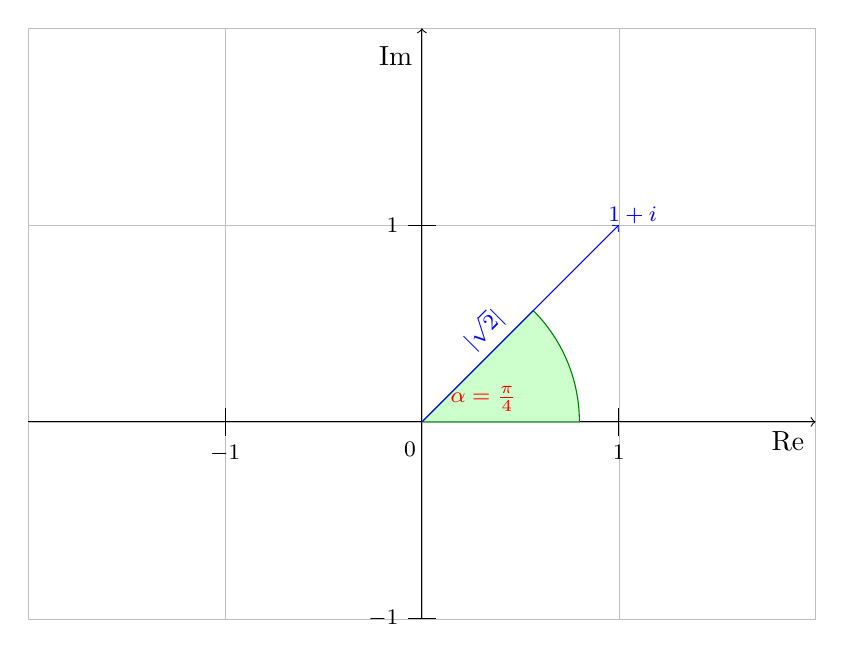
\begin{tikzpicture}[scale=2.5]

% Gitternetzlinien
\draw[xstep=1cm, ystep=1cm, very thin, color=lightgray] (-2,-1) grid (2,2);
% x-Achse
\draw[->] (-2,0) -- (2,0) node[below,xshift=-1em] {$\mathrm{Re}$}; 
%Zahlen auf x-Achse
\foreach \x in {-1,...,-1}
\draw[shift={(\x,0)},color=black] (0pt,2pt) -- (0pt,-2pt) node[below] {\footnotesize $\x$};
\foreach \x in {1,...,1}
\draw[shift={(\x,0)},color=black] (0pt,2pt) -- (0pt,-2pt) node[below] {\footnotesize $\x$};
% y-Achse 
\draw[->] (0,-1) -- (0,2) node[left,yshift=-1em] {$\mathrm{Im}$};%node[above left]
%Zahlen auf y-Achse
\foreach \y in {-1,...,-1}
\draw[shift={(0,\y)},color=black] (2pt,0pt) -- (-2pt,0pt) node[left] {\footnotesize $\y$};
\foreach \y in {1,...,1}
\draw[shift={(0,\y)},color=black] (2pt,0pt) -- (-2pt,0pt) node[left] {\footnotesize $\y$};
%Ursprung
%\draw[color=black] (0pt,-10pt) node[right] {\footnotesize $0$};
\draw[color=black] (-4pt,-4pt) node[right] {\footnotesize $0$};
%\draw[thick,color=black] plot[samples=200, domain=2:4] 
%(\x,{2}) node[below, xshift=-5em] {$h(x)$};

%\draw[thick,color=black] plot[samples=200, domain=-1:2] 
%(\x,{\x-1}) node[below, xshift=1em]{$g(x)$};

%\draw [blue] (0,0) circle (1);
\filldraw[fill=green!20,draw=green!50!black] (0,0) -- (8mm,0mm) arc (0:45:8mm) -- cycle; 
\draw [blue,->] (0,0)-.(1,1)node[below,xshift= 0.5em,yshift=1em] {\footnotesize $1+i$};
%\draw [blue,dashed] (0,.7)-.(0.7,0.7);
%\draw [blue,dashed] (0.7,0)-.(0.7,0.7);
%\draw [blue] (0.7,0) node[below,xshift= 0em,yshift=-0.2em] {\footnotesize $x$};
\draw [blue] (0.3,0.3) node[below,xshift= -0.5em,yshift=1.8em,rotate=45] {\footnotesize $|\sqrt{2}|$};
%\draw [blue] (0,0.7) node[below,xshift=- 0.51em,yshift=1em] {\footnotesize $y$};


%\draw [red,thick] (0,0)-.(0.7,0) node[midway,xshift= 0em,yshift=-0.5em] {\footnotesize $cos(\alpha)$};
%\draw [red,thick] (0,0)-.(0,0.7) node[midway,xshift= -0.50em,yshift=-0em,rotate=90] {\footnotesize $sin(\alpha)$};
\draw [red] (0.2,0.2) node[xshift= 0.8em,yshift=-0.6em,rotate=0] {\footnotesize $\alpha=\frac{\pi}{4}$};
\end{tikzpicture}\\
\end{center}
dann gilt:\\
\begin{align*}
(2+2\mathrm{i})^8=2^8=2^8\big(\sqrt{2}\big)^8\cdot \mathrm{e}^{\mathrm{i} \frac{\pi}{4}\cdot 8}=2^8 2^4 \mathrm{e}^{\mathrm{i}2\pi}=2^{12} \big(\underbrace {\mathrm{e}^{\mathrm{i}\pi}}_{=-1}\big)^2=4096\cdot (-1)^2=4096
\end{align*}
\subsubsection{ Aufgabe zur Multiplikation komplexer Zahlen in Polarkoordinaten}
\href{https://youtu.be/JumERKyIWbM}{Video 12}\\
Stelle die folgende komplexe Zahl in der Form von $ x+\mathrm{i}y $ dar:\\
\begin{align*}
(2+2\mathrm{i})^n+(2-2\mathrm{i})^n \text{ für } n\in \mathbb{N}
\end{align*}
\newpage
\noindent
\textbullet \;\; Umformung der komplexen Zahl:\\
\begin{quote}
	\begin{align*}
	(2+2\mathrm{i})^n+(2-2\mathrm{i})^n&=(2(1+\mathrm{i}))^n+(2(1-\mathrm{i}))^n\\
	                 &=2^n(1+\mathrm{i})^n+2^n(1-\mathrm{i})^n\\
	                 &=2^n \big((1+\mathrm{i})^n+(1-\mathrm{i})^n  \big)
	\end{align*}
\end{quote}
\textbullet \;\; Darstellung von $ (1+\mathrm{i}) $ und $ (1-\mathrm{i}) $ in Polarkoordinaten.\\
\begin{center}
	
	\begin{tikzpicture}[scale=2.5]
		\filldraw [->,draw=black,fill=red!20] (0,0)--(9mm,0mm) arc (0:315:9mm);
		\filldraw[->,draw=black,fill=green!20] (0,0) -- (7mm,0mm) arc (0:45:7mm); 
		\filldraw[->,fill=orange!20,draw=black,rotate=-45] (0,0) -- (8mm,0mm) arc (0:45:8mm); 
		
	% Gitternetzlinien
	\draw[xstep=1cm, ystep=1cm, very thin, color=lightgray] (-2,-2) grid (2,2);
	% x-Achse
	\draw[->] (-2,0) -- (2,0) node[below,xshift=-1em] {$\mathrm{\mathrm{Re}}$}; 
	%Zahlen auf x-Achse
	\foreach \x in {-1,...,-1}
	\draw[shift={(\x,0)},color=black] (0pt,2pt) -- (0pt,-2pt) node[below] {\footnotesize $\x$};
	\foreach \x in {1,...,1}
	\draw[shift={(\x,0)},color=black] (0pt,2pt) -- (0pt,-2pt) node[below] {\footnotesize $\x$};
	% y-Achse 
	\draw[->] (0,-2) -- (0,2) node[left,yshift=-1em] {$\mathrm{\mathrm{Im}}$};%node[above left]
	%Zahlen auf y-Achse
	\foreach \y in {-1,...,-1}
	\draw[shift={(0,\y)},color=black] (2pt,0pt) -- (-2pt,0pt) node[left] {\footnotesize $\y$};
	\foreach \y in {1,...,1}
	\draw[shift={(0,\y)},color=black] (2pt,0pt) -- (-2pt,0pt) node[left] {\footnotesize $\y$};
	%Ursprung
	\draw[color=black] (-4pt,-4pt) node[right] {\footnotesize $0$};
	

	\draw [blue,->] (0,0)-.(1,1)node[below,xshift= 0.5em,yshift=1em] {\footnotesize $1+\mathrm{i}$};

	\draw [blue,->] (0,0)-.(1,-1)node[below,xshift= 0.5em,yshift=1em] {\footnotesize $1-\mathrm{i}$};

	\draw [blue] (0.2,0.2) node[xshift= 0.8em,yshift=-0.6em,rotate=0] {\footnotesize $\alpha=\frac{\pi}{4}$};
	\draw [blue] (-0.2,-0.2) node[xshift= 3.8em,yshift=0.1em,rotate=0] {\footnotesize $\overset{\AC}{\alpha}=\frac{\pi}{4}$};
    \draw [blue] (-0.6,0.6) node[xshift= 1.3em,yshift=-0.9em,rotate=0] {\footnotesize $\beta=2\pi-\overset{\AC}{\alpha}$};
	 
	\end{tikzpicture}\\
\end{center}
\textbullet \;\; $ 1+\mathrm{i}=|1+\mathrm{i}|e^{\mathrm{i}\alpha}=\sqrt{2}\mathrm{e}^{\mathrm{i}\frac{\pi}{4}}$\\
\textbullet \;\; $ 1-\mathrm{i}=|1-\mathrm{i}|\mathrm{e}^{\mathrm{i}\beta} $\\
\begin{quote}
	$\beta=2\pi-\overset{\AC}{\alpha}=2\pi-\frac{\pi}{4}=\frac{7\pi}{4}  $\\
	$ 1-\mathrm{i}=\sqrt{2}\mathrm{e}^{\mathrm{i}\frac{7\pi}{4}} $
\end{quote}
Dann ist:\\
\begin{align*}
2^n \big((1+\mathrm{i})^n+(1-\mathrm{i})^n  \big)&=2^n \bigg(\big(\sqrt{2}\mathrm{e}^{\mathrm{i}\frac{\pi}{4}}\big)+\big(\sqrt{2} \mathrm{e}^{\mathrm{i}\frac{7\pi}{4}} \big)  \bigg)^n\\
&=2^n\big(2^{\frac{n}{2}}\mathrm{e}^{\mathrm{i}\cdot n\frac{\pi}{4}}+2^{\frac{n}{2}}\mathrm{e}^{\mathrm{i}\cdot n\frac{7\pi}{4}}\big)\\
&=2^{n+\frac{n}{2}}\big(\mathrm{e}^{\mathrm{i}\cdot n\frac{\pi}{4}}+\mathrm{e}^{\mathrm{i}\cdot n\frac{7\pi}{4}}\big)
\end{align*}
Es gilt: $\mathrm{e}^{\mathrm{i}\alpha}=\cos(\alpha)+\mathrm{i}\cdot \sin(\alpha)$\\
Dies eingesetzt ergibt:\\ 
\begin{align*}
2^n \big((1+\mathrm{i})^n+(1-\mathrm{i})^n  \big)&=2^{n+\frac{n}{2}}\big(\cos(\genfrac{}{}{}{2}{ n\pi}{ 4}) +\mathrm{i}\cdot \sin(\genfrac{}{}{}{2}{n\pi}{4})+ \cos(\genfrac{}{}{}{2}{  7 n \pi }{ 4}) +\mathrm{i}\cdot \sin(\genfrac{}{}{}{2}{ 7 n\pi  }{4})  \big)\\
&
\end{align*}
\begin{align*}
(2+2\mathrm{i})^n+(2-2\mathrm{i})^n=\underbrace {2^{n+\frac{n}{2}}\big(\cos(\genfrac{}{}{}{2}{n\pi }{4})+\cos(\genfrac{}{}{}{2}{ 7 n\pi  }{4}) \big)}_{x}+\underbrace {\mathrm{i} }_{\mathrm{i}}
\underbrace {2^{n+\frac{n}{2}}(sin(\genfrac{}{}{}{2}{n\pi}{4})+\sin(\genfrac{}{}{}{2}{ 7 n\pi }{4 }   )}_{y}
\end{align*}
\subsection{Wurzeln von komplexen Zahlen}
\href{https://youtu.be/5IVSZmGtt2Q}{Video 13}\\
Löse $ z^4=1 $:\\


\begin{center}
	Die Gleichung hat 4 Lösungen: $ z_1=1,z_2=\mathrm{i},z_3=-1,z_4=-\mathrm{i} $\vspace*{4mm}\\
	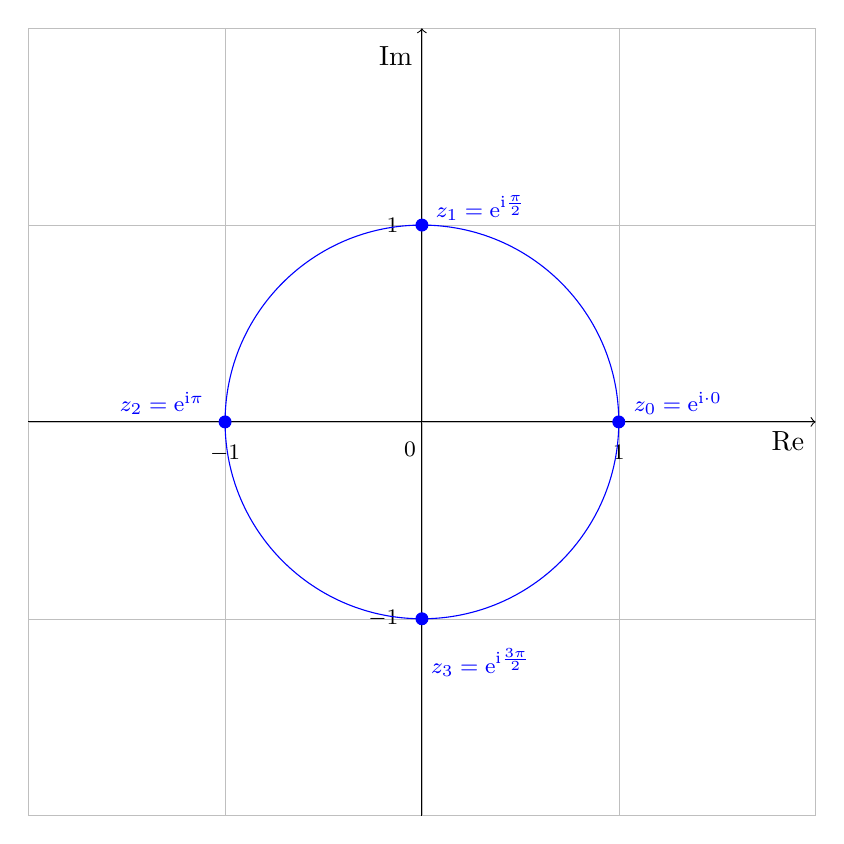
\begin{tikzpicture}[scale=2.5]
	
	% Gitternetzlinien
	\draw[xstep=1cm, ystep=1cm, very thin, color=lightgray] (-2,-2) grid (2,2);
	% x-Achse
	\draw[->] (-2,0) -- (2,0) node[below,xshift=-1em] {$\mathrm{Re}$}; 
	%Zahlen auf x-Achse
	\foreach \x in {-1,...,-1}
	\draw[shift={(\x,0)},color=black] (0pt,2pt) -- (0pt,-2pt) node[below] {\footnotesize $\x$};
	\foreach \x in {1,...,1}
	\draw[shift={(\x,0)},color=black] (0pt,2pt) -- (0pt,-2pt) node[below] {\footnotesize $\x$};
	% y-Achse 
	\draw[->] (0,-2) -- (0,2) node[left,yshift=-1em] {$\mathrm{Im}$};%node[above left]
	%Zahlen auf y-Achse
	\foreach \y in {-1,...,-1}
	\draw[shift={(0,\y)},color=black] (2pt,0pt) -- (-2pt,0pt) node[left] {\footnotesize $\y$};
	\foreach \y in {1,...,1}
	\draw[shift={(0,\y)},color=black] (2pt,0pt) -- (-2pt,0pt) node[left] {\footnotesize $\y$};
	%Ursprung
	%\draw[color=black] (0pt,-10pt) node[right] {\footnotesize $0$};
	\draw[color=black] (-4pt,-4pt) node[right] {\footnotesize $0$};
	%\draw[thick,color=black] plot[samples=200, domain=2:4] 
	%(\x,{2}) node[below, xshift=-5em] {$h(x)$};
	
	%\draw[thick,color=black] plot[samples=200, domain=-1:2] 
	%(\x,{\x-1}) node[below, xshift=1em]{$g(x)$};
	
	\draw [blue] (0,0) circle (1);
	%\filldraw[fill=green!20,draw=green!50!black] (0,0) -- (5mm,0mm) arc (0:45:5mm) -- cycle; 
	%\draw [blue,->] (0,0)-.(0.7,0.7)node[below,xshift= 0.5em,yshift=1em] {\footnotesize $z$};
	%\draw [blue,dashed] (0,.7)-.(0.7,0.7);
	%\draw [blue,dashed] (0.7,0)-.(0.7,0.7);
	%\draw [blue] (0.7,0) node[below,xshift= 0em,yshift=-0.2em] {\footnotesize $x$};
	%\draw [blue] (0.3,0.3) node[below,xshift= -0.5em,yshift=1.8em,rotate=45] {\footnotesize $|z|$};
	\draw [blue] (1.3,0.2) node[below,xshift=0em,yshift=0em] {\footnotesize $z_0=\mathrm{e}^{\mathrm{i}\cdot 0}$};
	\filldraw [blue] (1,0) circle (0.03);
	\draw [blue] (0.3,1.2) node[below,xshift=0em,yshift=0em] {\footnotesize $z_1=\mathrm{e}^{\mathrm{i}\frac{\pi}{2}}$};
	\filldraw [blue] (0,1) circle (0.03);
	\draw [blue] (-1.32,0.2) node[below,xshift=0em,yshift=0em] {\footnotesize $z_2=\mathrm{e}^{\mathrm{i}\pi}$};
	\filldraw [blue] (-1,0) circle (0.03);
	\draw [blue] (0.3,-1.1) node[below,xshift=0em,yshift=0em] {\footnotesize $z_3=\mathrm{e}^{\mathrm{i}\frac{3\pi}{2}}$};
	\filldraw [blue] (0,-1) circle (0.03);
	\end{tikzpicture}\\
\end{center}
es gilt:\\
\begin{align*}
z^4&=1=\mathrm{e}^{\mathrm{i}2\pi}\\
z&=\sqrt[4]{\mathrm{e}^{\mathrm{i}2\pi}}=\mathrm{e}^{\mathrm{i}\frac{2\pi}{4}}\\
\end{align*}
\begin{align*}
&z_0=\mathrm{e}^{\mathrm{i}\frac{2\pi}{4}\cdot 0}=\mathrm{e}^{\mathrm{i}\cdot 0}\\
&z_1=\mathrm{e}^{\mathrm{i}\frac{2\pi}{4}\cdot 1}=\mathrm{e}^{\mathrm{i}\frac{\pi}{2}}\\
&z_2=\mathrm{e}^{\mathrm{i}\frac{2\pi}{4}\cdot 2}=\mathrm{e}^{\mathrm{i}\pi}\\
&z_3=\mathrm{e}^{\mathrm{i}\frac{2\pi}{4}\cdot 3}=\mathrm{e}^{\mathrm{i}\frac{3\pi}{2}}\\
\end{align*}
Allgemein gilt dann:\\
Die Lösungen für $ z^n=1 $ sind:\\
\begin{center}
\boxed{z_k =\mathrm{e}^{\mathrm{i}\frac{2\pi\cdot k}{n}} \text{\;\;\;\;   für } k=0,1,2 \ldots n-1 }
\end{center}
\newpage
\noindent
\href{https://youtu.be/Uqpu2trEjM4}{Video 14}\\
Gegeben:\\$ z^n-a=0 $ für $ a\in  \mathbb{C} $\\
Gesucht: \\Alle Lösungen aus $  \mathbb{C}$\\
Es gilt:\\
\begin{align*}
&z^n=a=|a|e^{\mathrm{i}\alpha}\\
&z=\sqrt[n]{|a|}\mathrm{e}^{\mathrm{i} \frac{\alpha}{n}}
\end{align*}
Dies ist für den Winkel $ \alpha $ eine Lösung.\\
\begin{center}
	Die Gleichung hat k Lösungen an den Stellen: $ \mathrm{i}\frac{\alpha}{n}+\mathrm{i}\frac{2k\pi}{n}$ für $ k=0,1,2\ldots n-1 $\vspace*{4mm}\\
	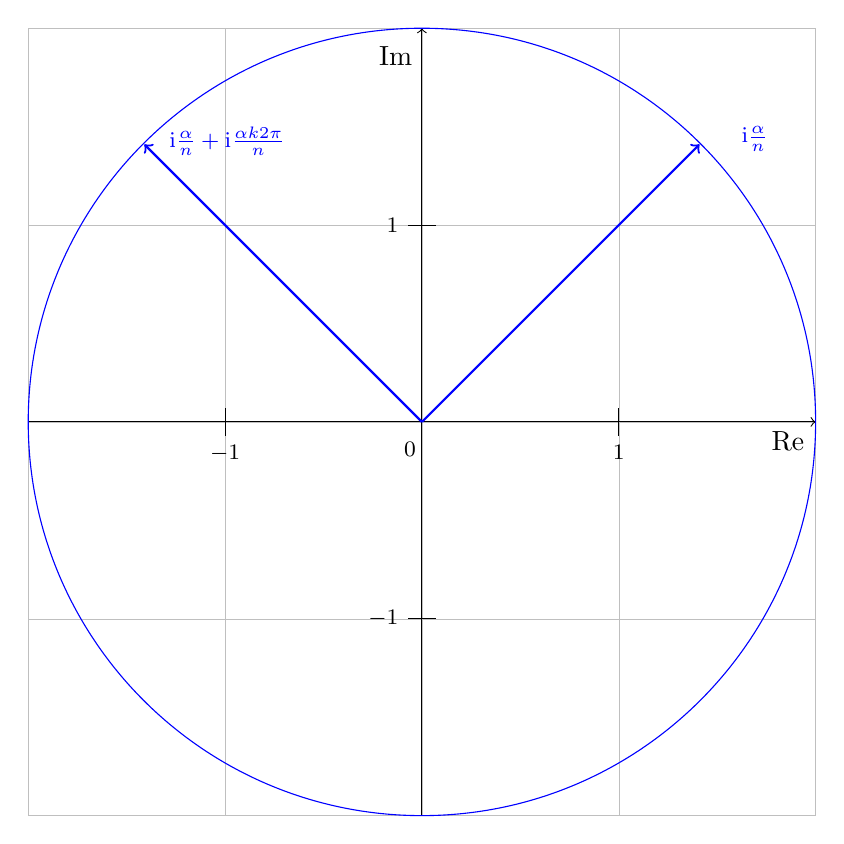
\begin{tikzpicture}[scale=2.5]
	
	% Gitternetzlinien
	\draw[xstep=1cm, ystep=1cm, very thin, color=lightgray] (-2,-2) grid (2,2);
	% x-Achse
	\draw[->] (-2,0) -- (2,0) node[below,xshift=-1em] {$\mathrm{Re}$}; 
	%Zahlen auf x-Achse
	\foreach \x in {-1,...,-1}
	\draw[shift={(\x,0)},color=black] (0pt,2pt) -- (0pt,-2pt) node[below] {\footnotesize $\x$};
	\foreach \x in {1,...,1}
	\draw[shift={(\x,0)},color=black] (0pt,2pt) -- (0pt,-2pt) node[below] {\footnotesize $\x$};
	% y-Achse 
	\draw[->] (0,-2) -- (0,2) node[left,yshift=-1em] {$\mathrm{Im}$};%node[above left]
	%Zahlen auf y-Achse
	\foreach \y in {-1,...,-1}
	\draw[shift={(0,\y)},color=black] (2pt,0pt) -- (-2pt,0pt) node[left] {\footnotesize $\y$};
	\foreach \y in {1,...,1}
	\draw[shift={(0,\y)},color=black] (2pt,0pt) -- (-2pt,0pt) node[left] {\footnotesize $\y$};
	%Ursprung
	%\draw[color=black] (0pt,-10pt) node[right] {\footnotesize $0$};
	\draw[color=black] (-4pt,-4pt) node[right] {\footnotesize $0$};
	%\draw[thick,color=black] plot[samples=200, domain=2:4] 
	%(\x,{2}) node[below, xshift=-5em] {$h(x)$};
	
	%\draw[thick,color=black] plot[samples=200, domain=-1:2] 
	%(\x,{\x-1}) node[below, xshift=1em]{$g(x)$};
	
	\draw [blue] (0,0) circle (2);
	%\filldraw[fill=green!20,draw=green!50!black] (0,0) -- (5mm,0mm) arc (0:45:5mm) -- cycle; 
	%\draw [blue,->] (0,0)-.(0.7,0.7)node[below,xshift= 0.5em,yshift=1em] {\footnotesize $z$};
	%\draw [blue,dashed] (0,.7)-.(0.7,0.7);
	%\draw [blue,dashed] (0.7,0)-.(0.7,0.7);
	%\draw [blue] (0.7,0) node[below,xshift= 0em,yshift=-0.2em] {\footnotesize $x$};
	%\draw [blue] (0.3,0.3) node[below,xshift= -0.5em,yshift=1.8em,rotate=45] {\footnotesize $|z|$};
	\draw [blue] (1.41,1.41) node[below,xshift=2em,yshift=1em] {\footnotesize $\mathrm{i}\frac{\alpha}{n}$};
	\draw [blue,->,thick] (0,0)--(1.41,1.41);
	\draw [blue] (-1.41,1.41) node[below,xshift=3em,yshift=1em] {\footnotesize $\mathrm{i}\frac{\alpha}{n}+\mathrm{i}\frac{\alpha k 2\pi}{n}$};
	\draw [blue,->,thick] (0,0)--(-1.41,1.41);
	%\filldraw [blue] (1.41,1.41) circle (0.03);
	
	\end{tikzpicture}\\
\end{center}
\begin{align*}
 \boxed{z_k=\sqrt[n]{|a|}\cdot \mathrm{e}^{\mathrm{i}\frac{\alpha}{n}+\mathrm{i}\frac{2k\pi}{n}}\;\;\;\;\text{für } k=0,1,2\ldots n-1}
\end{align*}
Beispiel:\\
Gegeben: $ z^3=2\mathrm{i} $\\
Gesucht: Alle Lösungen aus $  \mathbb{C} $\\
Es gilt:\\
\begin{align*}
z^3=2\mathrm{i}=0+2\mathrm{i}=|2|\mathrm{e}^{\mathrm{i}\alpha}
\end{align*}
\newpage
\noindent
Winkel $ \alpha $ bestimmen:\vspace*{2mm}\\
\begin{center}
	
	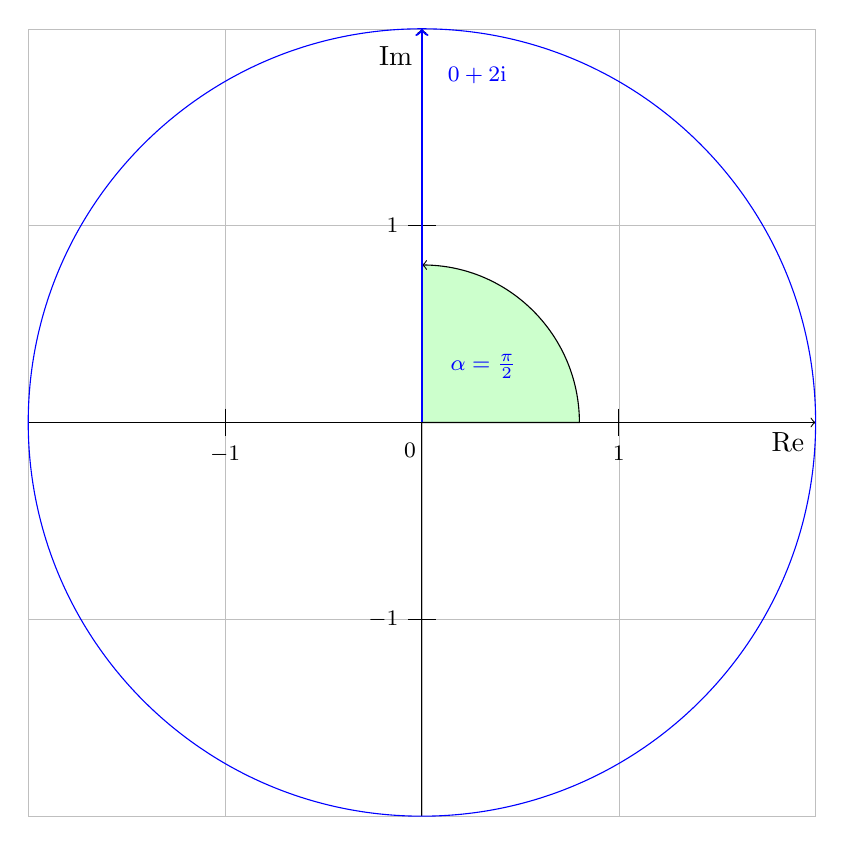
\begin{tikzpicture}[scale=2.5]
	
	% Gitternetzlinien
	\draw[xstep=1cm, ystep=1cm, very thin, color=lightgray] (-2,-2) grid (2,2);
	% x-Achse
	\draw[->] (-2,0) -- (2,0) node[below,xshift=-1em] {$\mathrm{Re}$}; 
	%Zahlen auf x-Achse
	\foreach \x in {-1,...,-1}
	\draw[shift={(\x,0)},color=black] (0pt,2pt) -- (0pt,-2pt) node[below] {\footnotesize $\x$};
	\foreach \x in {1,...,1}
	\draw[shift={(\x,0)},color=black] (0pt,2pt) -- (0pt,-2pt) node[below] {\footnotesize $\x$};
	% y-Achse 
	\draw[->] (0,-2) -- (0,2) node[left,yshift=-1em] {$\mathrm{Im}$};%node[above left]
	%Zahlen auf y-Achse
	\foreach \y in {-1,...,-1}
	\draw[shift={(0,\y)},color=black] (2pt,0pt) -- (-2pt,0pt) node[left] {\footnotesize $\y$};
	\foreach \y in {1,...,1}
	\draw[shift={(0,\y)},color=black] (2pt,0pt) -- (-2pt,0pt) node[left] {\footnotesize $\y$};
	%Ursprung
	%\draw[color=black] (0pt,-10pt) node[right] {\footnotesize $0$};
	\draw[color=black] (-4pt,-4pt) node[right] {\footnotesize $0$};
	%\draw[thick,color=black] plot[samples=200, domain=2:4] 
	%(\x,{2}) node[below, xshift=-5em] {$h(x)$};
	
	%\draw[thick,color=black] plot[samples=200, domain=-1:2] 
	%(\x,{\x-1}) node[below, xshift=1em]{$g(x)$};
	
	\draw [blue] (0,0) circle (2);
	\filldraw[->,draw=black,fill=green!20] (0,0) -- (8mm,0mm) arc (0:90:8mm); 
	%\filldraw[->,fill=green!20,draw=green!50!black] (0,0) -- (9mm,0mm) arc (0:90:9mm) -- cycle; 
	\draw [blue] (0.2,0.2) node[xshift= 0.8em,yshift=0.6em,rotate=0] {\footnotesize $\alpha=\frac{\pi}{2}$};
	%\draw [blue,->] (0,0)-.(0.7,0.7)node[below,xshift= 0.5em,yshift=1em] {\footnotesize $z$};
	%\draw [blue,dashed] (0,.7)-.(0.7,0.7);
	%\draw [blue,dashed] (0.7,0)-.(0.7,0.7);
	%\draw [blue] (0.7,0) node[below,xshift= 0em,yshift=-0.2em] {\footnotesize $x$};
	%\draw [blue] (0.3,0.3) node[below,xshift= -0.5em,yshift=1.8em,rotate=45] {\footnotesize $|z|$};
	\draw [blue] (0,2) node[below,xshift=2em,yshift=-1em] {\footnotesize $0+2\mathrm{i}$};
	\draw [blue,->,thick] (0,0)--(0,2);
	%\draw [blue] (-1.41,1.41) node[below,xshift=3em,yshift=1em] {\footnotesize $i\frac{\alpha}{n}+i\frac{\alpha k 2\pi}{n}$};
	%\draw [blue,->] (0,0)--(-1.41,1.41);
	%\filldraw [blue] (1.41,1.41) circle (0.03);
	
	\end{tikzpicture}\\
\end{center}
Winkel $ \alpha=\frac{\pi}{2} $
also gilt:
\begin{align*}
z^3=|2|\mathrm{e}^{\mathrm{i}\frac{\pi}{2}}
\end{align*}
D.h.:\\
\begin{align*}
z_k=\sqrt[3]{2}\cdot \mathrm{e}^{\mathrm{i} \frac{\pi}{2\cdot 3}+\mathrm{i}\frac{2k\pi}{3}}\;\;\;\;\text{für } k=0,1,2 \ldots n-1
\end{align*}
\subsubsection{Aufgabe zum Thema komplexe Lösungen von Gleichungen}
\href{https://youtu.be/UOdKG8lbwiQ}{Video 15}\\
Berechne alle Lösungen von:\\
\begin{tabular}[t]{lll}% l=linksbündig r=rechtsbündig
	(i) & $z^5=3\mathrm{i}+3  $  \\
	(ii) & $z^7=16\mathrm{i}-16  $ \\
	(iii)&$ \mathrm{i}z-\overline{z} =4$	
\end{tabular} \vspace*{6mm}\\
(i)\;\;$ z^5=3\mathrm{i}+3 $\\
\begin{quote}
Es gilt:\\
\begin{align*}
z^5=3\mathrm{i}+3=3(1+\mathrm{i})=3\sqrt{1^2+1^2}\;\;\mathrm{e}^{\mathrm{i}\alpha}
\end{align*}
\begin{center}
	Winkel $ \alpha $ bestimmen:\vspace*{2mm}\\
	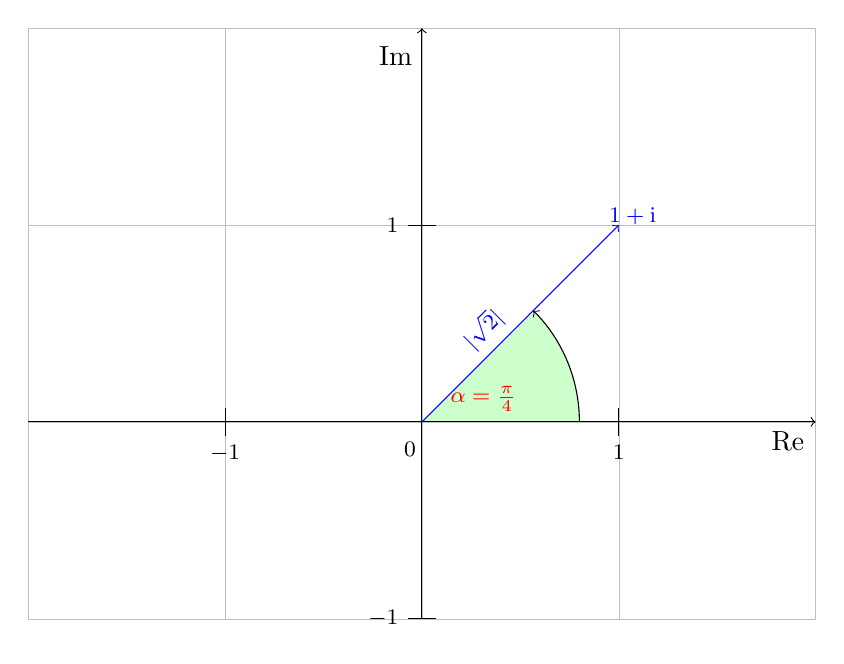
\begin{tikzpicture}[scale=2.5]
	\filldraw[->,draw=black,fill=green!20] (0,0) -- (8mm,0mm) arc (0:45:8mm); 
	% Gitternetzlinien
	\draw[xstep=1cm, ystep=1cm, very thin, color=lightgray] (-2,-1) grid (2,2);
	% x-Achse
	\draw[->] (-2,0) -- (2,0) node[below,xshift=-1em] {$\mathrm{Re}$}; 
	%Zahlen auf x-Achse
	\foreach \x in {-1,...,-1}
	\draw[shift={(\x,0)},color=black] (0pt,2pt) -- (0pt,-2pt) node[below] {\footnotesize $\x$};
	\foreach \x in {1,...,1}
	\draw[shift={(\x,0)},color=black] (0pt,2pt) -- (0pt,-2pt) node[below] {\footnotesize $\x$};
	% y-Achse 
	\draw[->] (0,-1) -- (0,2) node[left,yshift=-1em] {$\mathrm{Im}$};%node[above left]
	%Zahlen auf y-Achse
	\foreach \y in {-1,...,-1}
	\draw[shift={(0,\y)},color=black] (2pt,0pt) -- (-2pt,0pt) node[left] {\footnotesize $\y$};
	\foreach \y in {1,...,1}
	\draw[shift={(0,\y)},color=black] (2pt,0pt) -- (-2pt,0pt) node[left] {\footnotesize $\y$};
	%Ursprung
	%\draw[color=black] (0pt,-10pt) node[right] {\footnotesize $0$};
	\draw[color=black] (-4pt,-4pt) node[right] {\footnotesize $0$};
	%\draw[thick,color=black] plot[samples=200, domain=2:4] 
	%(\x,{2}) node[below, xshift=-5em] {$h(x)$};
	
	%\draw[thick,color=black] plot[samples=200, domain=-1:2] 
	%(\x,{\x-1}) node[below, xshift=1em]{$g(x)$};
	
	%\draw [blue] (0,0) circle (1);
	%\filldraw[fill=green!20,draw=green!50!black] (0,0) -- (8mm,0mm) arc (0:45:8mm) -- cycle; 
	\draw [blue,->] (0,0)-.(1,1)node[below,xshift= 0.5em,yshift=1em] {\footnotesize $1+\mathrm{i}$};
	%\draw [blue,dashed] (0,.7)-.(0.7,0.7);
	%\draw [blue,dashed] (0.7,0)-.(0.7,0.7);
	%\draw [blue] (0.7,0) node[below,xshift= 0em,yshift=-0.2em] {\footnotesize $x$};
	\draw [blue] (0.3,0.3) node[below,xshift= -0.5em,yshift=1.8em,rotate=45] {\footnotesize $|\sqrt{2}|$};
	%\draw [blue] (0,0.7) node[below,xshift=- 0.51em,yshift=1em] {\footnotesize $y$};
	
	
	%\draw [red,thick] (0,0)-.(0.7,0) node[midway,xshift= 0em,yshift=-0.5em] {\footnotesize $cos(\alpha)$};
	%\draw [red,thick] (0,0)-.(0,0.7) node[midway,xshift= -0.50em,yshift=-0em,rotate=90] {\footnotesize $sin(\alpha)$};
	\draw [red] (0.2,0.2) node[xshift= 0.8em,yshift=-0.6em,rotate=0] {\footnotesize $\alpha=\frac{\pi}{4}$};
	\end{tikzpicture}\\
\end{center}
\begin{align*}
z^5=3\sqrt{2}\;\;\mathrm{e}^{\mathrm{i}\frac{\pi}{4}}
\end{align*}
Lösungen sind:\\
\begin{align*}
z_k=\sqrt[5]{\scriptscriptstyle 3\sqrt{2}}\;\;\mathrm{e}^{\mathrm{i}\frac{\pi}{5\cdot4}+\mathrm{i}\frac{2\pi k}{5}}=\sqrt[5]{\scriptscriptstyle 3\sqrt{2}}\;\;\mathrm{e}^{\mathrm{i}\frac{\pi}{20}+\mathrm{i}\frac{2\pi k}{5}}\;\;\;\text{für } k=0,1,2\ldots n-1
\end{align*}
\end{quote}
(ii)\;\;$ z^7=16\mathrm{i}-16 $\\
\begin{quote}
	
\begin{align*}
 z^7=16\mathrm{i}-16=16(-1+\mathrm{i})=16\sqrt{2}\;\;\mathrm{e}^{\mathrm{i}\alpha}
\end{align*}
\begin{center}
	Winkel $ \alpha $ bestimmen:\vspace*{2mm}\\
	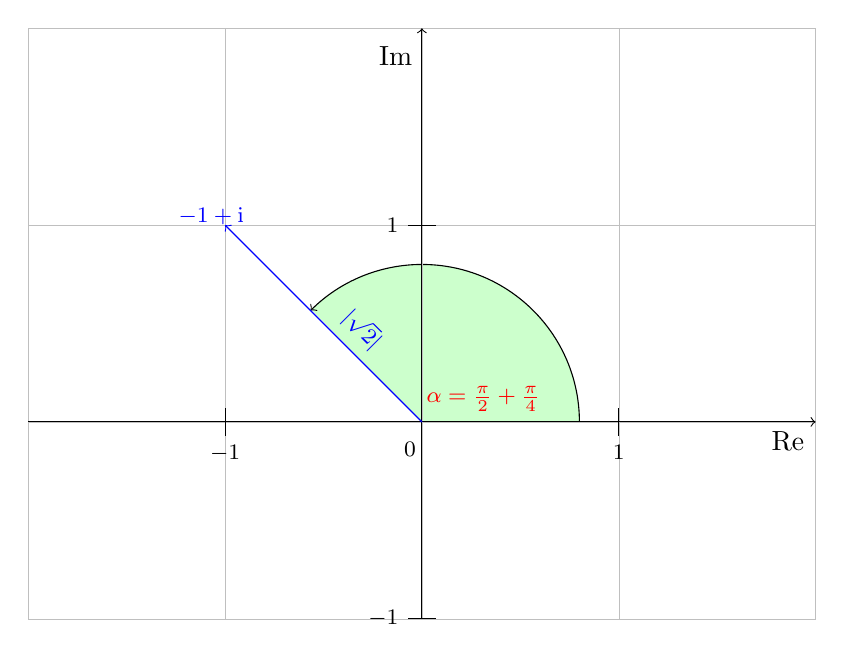
\begin{tikzpicture}[scale=2.5]
	\filldraw[->,draw=black,fill=green!20] (0,0) -- (8mm,0mm) arc (0:135:8mm); 
	% Gitternetzlinien
	\draw[xstep=1cm, ystep=1cm, very thin, color=lightgray] (-2,-1) grid (2,2);
	% x-Achse
	\draw[->] (-2,0) -- (2,0) node[below,xshift=-1em] {$\mathrm{Re}$}; 
	%Zahlen auf x-Achse
	\foreach \x in {-1,...,-1}
	\draw[shift={(\x,0)},color=black] (0pt,2pt) -- (0pt,-2pt) node[below] {\footnotesize $\x$};
	\foreach \x in {1,...,1}
	\draw[shift={(\x,0)},color=black] (0pt,2pt) -- (0pt,-2pt) node[below] {\footnotesize $\x$};
	% y-Achse 
	\draw[->] (0,-1) -- (0,2) node[left,yshift=-1em] {$\mathrm{Im}$};%node[above left]
	%Zahlen auf y-Achse
	\foreach \y in {-1,...,-1}
	\draw[shift={(0,\y)},color=black] (2pt,0pt) -- (-2pt,0pt) node[left] {\footnotesize $\y$};
	\foreach \y in {1,...,1}
	\draw[shift={(0,\y)},color=black] (2pt,0pt) -- (-2pt,0pt) node[left] {\footnotesize $\y$};
	%Ursprung
	%\draw[color=black] (0pt,-10pt) node[right] {\footnotesize $0$};
	\draw[color=black] (-4pt,-4pt) node[right] {\footnotesize $0$};
	
	
	\draw [blue,->] (0,0)-.(-1,1)node[below,xshift= -0.5em,yshift=1em] {\footnotesize $-1+\mathrm{i}$};

	\draw [blue] (-0.15,0.3) node[below,xshift= -0.5em,yshift=1.8em,rotate=-45] {\footnotesize $|\sqrt{2}|$};

	\draw [red] (0.2,0.2) node[xshift= 0.8em,yshift=-0.6em,rotate=0] {\footnotesize $\alpha=\frac{\pi}{2}+\frac{\pi}{4}$};
	\end{tikzpicture}\\
\end{center}
\begin{align*}
z^7=16\sqrt{2}\;\;\mathrm{e}^{\mathrm{i}\frac{3}{4}\pi}
\end{align*}
Lösungen sind:\\
\begin{align*}
z_k=\sqrt[7]{\scriptscriptstyle 16\sqrt{2}}\;\;\mathrm{e}^{\mathrm{i}\frac{3\pi}{4\cdot7}+\frac{2\pi k}{7}}=\sqrt[7]{\scriptscriptstyle 16\sqrt{2}}\;\;\mathrm{e}^{\mathrm{i}\frac{3\pi}{28}+\frac{2\pi k}{7}}\;\;\;\;\text{für }k=0,1,2\ldots n-1
\end{align*}
\end{quote}
(iii)\;\; $\mathrm{i}z-\mathrm{i} \overline{z}=4$\\
\begin{quote}
Es gilt mit: $ z=x+\mathrm{i}y $\\
	\begin{center}
	
	\begin{tabular}[t]{r@{$=$}ll}% l=linksbündig r=rechtsbündig
		$\mathrm{i}(x+\mathrm{i}y)-\mathrm{i}(x-\mathrm{i}y)$ & $4$\\
		$\mathrm{i}x+\mathrm{i}^2y-\mathrm{i}x+\mathrm{i}^2y$ & $4 $ \\	
		$ -2y $&$ 4 $\\
		$ y $&$-2  $ und $ x $ beliebig\\
	\end{tabular} \\
\end{center}
Lösung:$ \{ x+\mathrm{i}y\;|\;x\in \mathbb{R}\wedge y=-2\} $
\end{quote}

\subsection{Bestimmung des Winkels bei Polarkoordinaten}
\href{https://youtu.be/FokqSBZakd4}{Video 16}\\
Sei $z \in \mathbb{C}\setminus\{0\} $ und $ z=x+\mathrm{i}y=|z|\;\mathrm{e}^{\mathrm{i}\alpha} $\vspace*{2mm}\\
Wie bestimmt man den Winkel $ \alpha $ ?\\
\begin{center}
	\begin{align*}
	z=|z|(\cos(\alpha)+\mathrm{i}\;\sin(\alpha))
	\end{align*}
	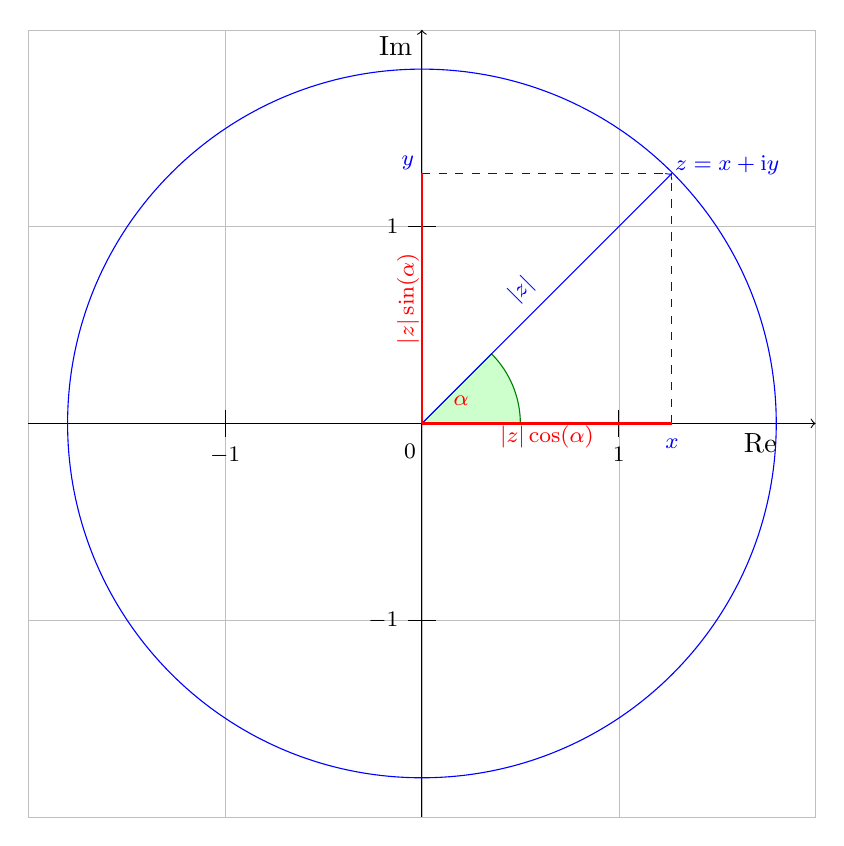
\begin{tikzpicture}[scale=2.5]
	
	% Gitternetzlinien
	\draw[xstep=1cm, ystep=1cm, very thin, color=lightgray] (-2,-2) grid (2,2);
	% x-Achse
	\draw[->] (-2,0) -- (2,0) node[below,xshift=-2em] {$\mathrm{Re}$}; 
	%Zahlen auf x-Achse
	\foreach \x in {-1,...,-1}
	\draw[shift={(\x,0)},color=black] (0pt,2pt) -- (0pt,-2pt) node[below] {\footnotesize $\x$};
	\foreach \x in {1,...,1}
	\draw[shift={(\x,0)},color=black] (0pt,2pt) -- (0pt,-2pt) node[below] {\footnotesize $\x$};
	% y-Achse 
	\draw[->] (0,-2) -- (0,2) node[left,yshift=-0.6em] {$\mathrm{Im}$};%node[above left]
	%Zahlen auf y-Achse
	\foreach \y in {-1,...,-1}
	\draw[shift={(0,\y)},color=black] (2pt,0pt) -- (-2pt,0pt) node[left] {\footnotesize $\y$};
	\foreach \y in {1,...,1}
	\draw[shift={(0,\y)},color=black] (2pt,0pt) -- (-2pt,0pt) node[left] {\footnotesize $\y$};
	%Ursprung
	%\draw[color=black] (0pt,-10pt) node[right] {\footnotesize $0$};
	\draw[color=black] (-4pt,-4pt) node[right] {\footnotesize $0$};
	%\draw[thick,color=black] plot[samples=200, domain=2:4] 
	%(\x,{2}) node[below, xshift=-5em] {$h(x)$};
	
	%\draw[thick,color=black] plot[samples=200, domain=-1:2] 
	%(\x,{\x-1}) node[below, xshift=1em]{$g(x)$};
	
	\draw [blue] (0,0) circle (1.8);
	\filldraw[fill=green!20,draw=green!50!black] (0,0) -- (5mm,0mm) arc (0:45:5mm) -- cycle; 
	\draw [blue,->] (0,0)-.(1.27,1.27)node[below,xshift= 2em,yshift=1em] {\footnotesize $z=x+\mathrm{i}y$};
	\draw [blue,dashed] (0,1.27)-.(1.27,1.27);
	\draw [blue,dashed] (1.27,0)-.(1.27,1.27);
	\draw [blue] (1.27,0) node[below,xshift= 0em,yshift=-0.2em] {\footnotesize $x$};
	\draw [blue] (0.5,0.5) node[below,xshift= -0.5em,yshift=1.8em,rotate=45] {\footnotesize $|z|$};
	\draw [blue] (0,1.27) node[below,xshift=- 0.51em,yshift=1em] {\footnotesize $y$};
	
	
	\draw [red,thick] (0,0)-.(1.27,0) node[midway,xshift= 0em,yshift=-0.5em] {\footnotesize $|z|\cos(\alpha)$};
	\draw [red,thick] (0,0)-.(0,1.27) node[midway,xshift= -0.50em,yshift=0em,rotate=90] {\footnotesize $|z|\sin(\alpha)$};
	\draw [red] (0.2,0.2) node[xshift= 0em,yshift=-0.6em,rotate=0] {\footnotesize $\alpha$};
	\end{tikzpicture}\\
\end{center}
Die Umkehrfunktion von $ \cos(\alpha) $ bzw. $ \sin(\alpha) $ sind:\\
\begin{align*}
&\arccos: [-1,1]\longmapsto [0,\pi]\\
&\arcsin: [-1,1]\longmapsto [\scriptscriptstyle -\genfrac{}{}{}{\pi}{\pi}{2 },\genfrac{}{}{}{2}{\pi}{2 }\displaystyle ]
\end{align*}
Dann gilt:\\
\begin{align*}
&x=|z|\cos(\alpha)\Leftrightarrow \cos(\alpha)=\frac{x}{|z|}&y=|z|sin(\alpha)\Leftrightarrow \cos(\alpha)=\frac{y}{|z|}\\
&\alpha=\arccos \bigg(\frac{x}{|z| }\bigg)
&\alpha=\arcsin \bigg(\frac{y }{|z| }\bigg)\\
\end{align*}
Bemerkung:\\
Falsch ist:\\
\begin{align*}
\alpha=\arccos(\genfrac{}{}{}{2}{x}{|z| })=\arcsin(\genfrac{}{}{}{2}{y}{|z| })
\end{align*}
Weil die Abbildung vom arccos $[0,\pi]  $ ist und vom arcsin $ [\scriptscriptstyle -\genfrac{}{}{}{\pi}{\pi}{2 },\genfrac{}{}{}{2}{\pi}{2 }\displaystyle ] $ ist. \vspace*{4mm}\\
\textbullet \;\; für $ \alpha [0,\pi]$ gilt:\\

\begin{center}
$ \alpha=\arccos(\genfrac{}{}{}{2}{x }{|z| }) $ für $[0,\pi]$\\
	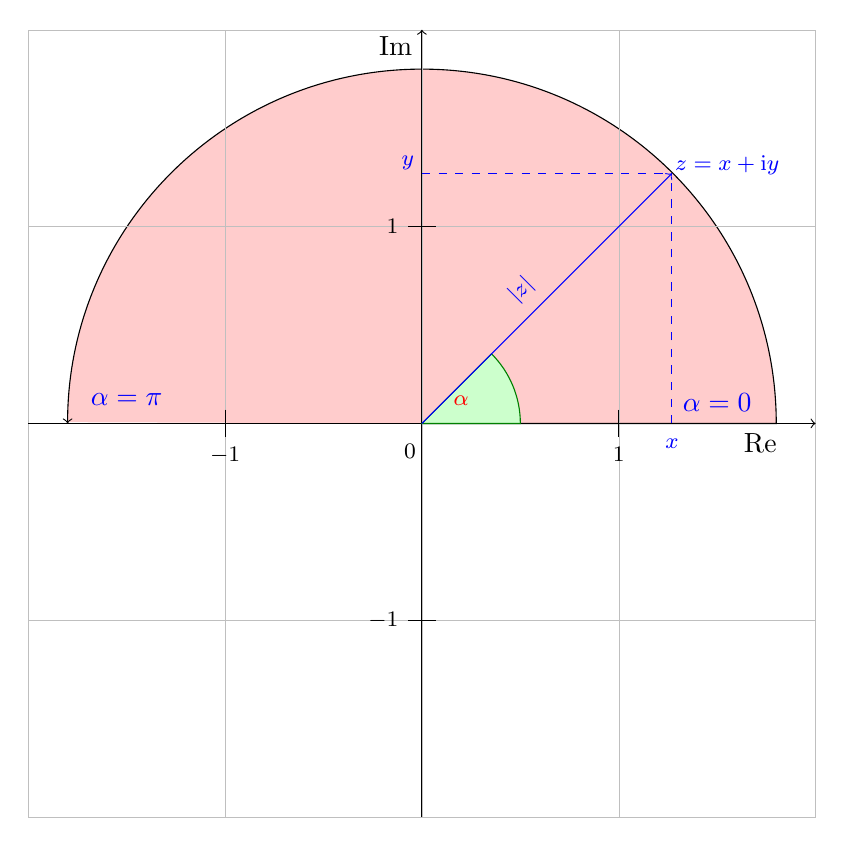
\begin{tikzpicture}[scale=2.5]
	\filldraw [->,draw=black,fill=red!20] (0,0)--(18mm,0mm) arc (0:180:18mm);
	% Gitternetzlinien
	\draw[xstep=1cm, ystep=1cm, very thin, color=lightgray] (-2,-2) grid (2,2);
	% x-Achse
	\draw[->] (-2,0) -- (2,0) node[below,xshift=-2em] {$\mathrm{Re}$}; 
	%Zahlen auf x-Achse
	\foreach \x in {-1,...,-1}
	\draw[shift={(\x,0)},color=black] (0pt,2pt) -- (0pt,-2pt) node[below] {\footnotesize $\x$};
	\foreach \x in {1,...,1}
	\draw[shift={(\x,0)},color=black] (0pt,2pt) -- (0pt,-2pt) node[below] {\footnotesize $\x$};
	% y-Achse 
	\draw[->] (0,-2) -- (0,2) node[left,yshift=-0.6em] {$\mathrm{Im}$};%node[above left]
	%Zahlen auf y-Achse
	\foreach \y in {-1,...,-1}
	\draw[shift={(0,\y)},color=black] (2pt,0pt) -- (-2pt,0pt) node[left] {\footnotesize $\y$};
	\foreach \y in {1,...,1}
	\draw[shift={(0,\y)},color=black] (2pt,0pt) -- (-2pt,0pt) node[left] {\footnotesize $\y$};
	%Ursprung
	%\draw[color=black] (0pt,-10pt) node[right] {\footnotesize $0$};
	\draw[color=black] (-4pt,-4pt) node[right] {\footnotesize $0$};
	%\draw[thick,color=black] plot[samples=200, domain=2:4] 
	%(\x,{2}) node[below, xshift=-5em] {$h(x)$};
	
	%\draw[thick,color=black] plot[samples=200, domain=-1:2] 
	%(\x,{\x-1}) node[below, xshift=1em]{$g(x)$};
	
	%\draw [blue] (0,0) circle (1.8);
	\filldraw[fill=green!20,draw=green!50!black] (0,0) -- (5mm,0mm) arc (0:45:5mm) -- cycle; 
	\draw [blue,->] (0,0)-.(1.27,1.27)node[below,xshift= 2em,yshift=1em] {\footnotesize $z=x+\mathrm{i}y$};
	\draw [blue,dashed] (0,1.27)-.(1.27,1.27);
	\draw [blue,dashed] (1.27,0)-.(1.27,1.27);
	\draw [blue] (1.27,0) node[below,xshift= 0em,yshift=-0.2em] {\footnotesize $x$};
	\draw [blue] (0.5,0.5) node[below,xshift= -0.5em,yshift=1.8em,rotate=45] {\footnotesize $|z|$};
	\draw [blue] (0,1.27) node[below,xshift=- 0.51em,yshift=1em] {\footnotesize $y$};
	
	
	
	\draw [red] (0.2,0.2) node[xshift= 0em,yshift=-0.6em,rotate=0] {\footnotesize $\alpha$};
		%\draw[->,draw=green] (0,0) -- (18mm,0mm) arc (0:180:18mm) -- cycle; 
	\draw [blue] (-1.5,.2) node[below,xshift=- 0em,yshift=0em] { $\alpha=\pi$};
	\draw [blue] (1.5,.2) node[below,xshift=- 0em,yshift=0em] { $\alpha=0$};
	\end{tikzpicture}\\
\end{center}
\newpage
\noindent
\textbullet \;\; für $ \alpha ]\pi,2\pi[ $ gilt:\\

\begin{center}
	$ \alpha=2\pi-\arccos(\genfrac{}{}{}{2}{x }{|z| }) $ für $]\pi,2\pi[  $\\
	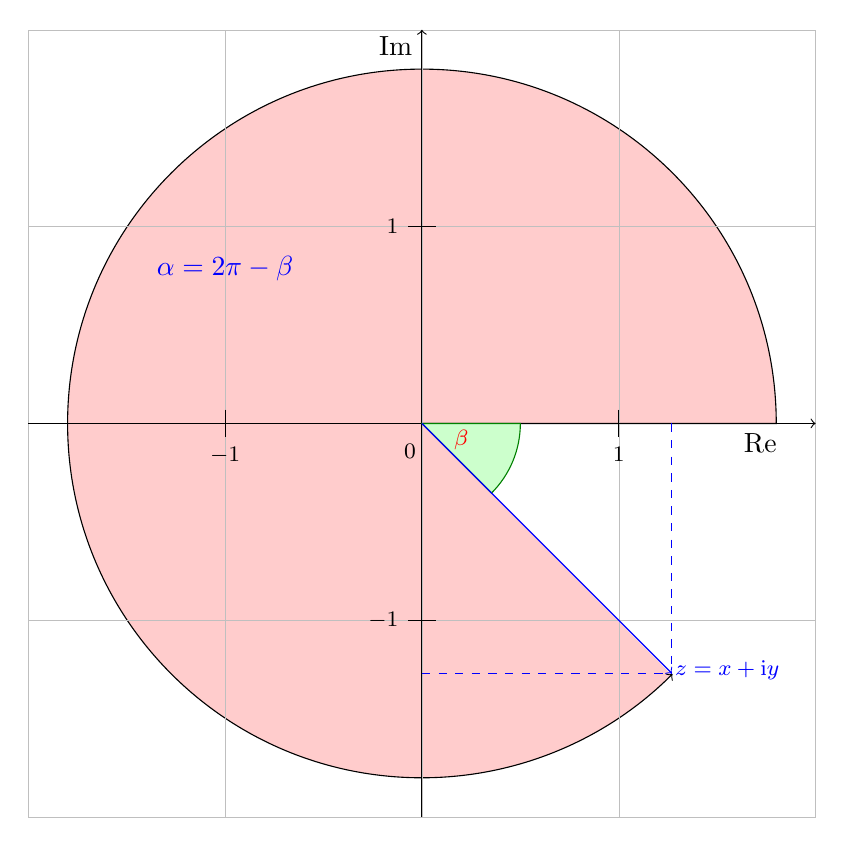
\begin{tikzpicture}[scale=2.5]
	\filldraw [->,draw=black,fill=red!20] (0,0)--(18mm,0mm) arc (0:315:18mm);
	% Gitternetzlinien
	\draw[xstep=1cm, ystep=1cm, very thin, color=lightgray] (-2,-2) grid (2,2);
	% x-Achse
	\draw[->] (-2,0) -- (2,0) node[below,xshift=-2em] {$\mathrm{Re}$}; 
	%Zahlen auf x-Achse
	\foreach \x in {-1,...,-1}
	\draw[shift={(\x,0)},color=black] (0pt,2pt) -- (0pt,-2pt) node[below] {\footnotesize $\x$};
	\foreach \x in {1,...,1}
	\draw[shift={(\x,0)},color=black] (0pt,2pt) -- (0pt,-2pt) node[below] {\footnotesize $\x$};
	% y-Achse 
	\draw[->] (0,-2) -- (0,2) node[left,yshift=-0.6em] {$\mathrm{Im}$};%node[above left]
	%Zahlen auf y-Achse
	\foreach \y in {-1,...,-1}
	\draw[shift={(0,\y)},color=black] (2pt,0pt) -- (-2pt,0pt) node[left] {\footnotesize $\y$};
	\foreach \y in {1,...,1}
	\draw[shift={(0,\y)},color=black] (2pt,0pt) -- (-2pt,0pt) node[left] {\footnotesize $\y$};
	%Ursprung
	%\draw[color=black] (0pt,-10pt) node[right] {\footnotesize $0$};
	\draw[color=black] (-4pt,-4pt) node[right] {\footnotesize $0$};
	%\draw[thick,color=black] plot[samples=200, domain=2:4] 
	%(\x,{2}) node[below, xshift=-5em] {$h(x)$};
	
	%\draw[thick,color=black] plot[samples=200, domain=-1:2] 
	%(\x,{\x-1}) node[below, xshift=1em]{$g(x)$};
	
	%\draw [blue] (0,0) circle (1.8);
	\filldraw[fill=green!20,draw=green!50!black] (0,0) -- (5mm,0mm) arc (0:-45:5mm) -- cycle; 
	\draw [blue,->] (0,0)-.(1.27,-1.27)node[below,xshift= 2em,yshift=0.8em] {\footnotesize $z=x+\mathrm{i}y$};
	\draw [blue,dashed] (0,-1.27)-.(1.27,-1.27);
	\draw [blue,dashed] (1.27,0)-.(1.27,-1.27);
	%\draw [blue] (1.27,0) node[below,xshift= 0em,yshift=-0.2em] {\footnotesize $x$};
	%\draw [blue] (-0.5,0.9) node[below,xshift= -0.5em,yshift=1.8em,rotate=45] {\footnotesize $|z|$};
	%\draw [blue] (0,1.27) node[below,xshift=- 0.51em,yshift=1em] {\footnotesize $y$};
	
	
	
	\draw [red] (0.2,-0) node[xshift= 0em,yshift=-0.6em,rotate=0] {\footnotesize $\beta$};
	%\draw[->,draw=green] (0,0) -- (18mm,0mm) arc (0:180:18mm) -- cycle; 
	\draw [blue] (-1,0.9) node[below,xshift=- 0em,yshift=0em] { $\alpha=2\pi-\beta$};
	%\draw [blue] (1.5,.2) node[below,xshift=- 0em,yshift=0em] { $\alpha=0$};
	\end{tikzpicture}\\
\end{center}